\documentclass[12pt,a4paper]{book}

% $Id: pyvisi_doc.tex,v 1.3 2005/02/07 06:06:57 paultcochrane Exp $

%\setcounter{secnumdepth}{4}
%\setcounter{tocdepth}{4}

% $Id: pyvisi_defs.tex,v 1.2 2005/01/12 06:37:55 paultcochrane Exp $

\usepackage{html}
\usepackage{xspace}
% \usepackage{verbatim}  % better implementation of verbatim environment
\usepackage{alltt} % a verbatim-like environment that accepts commands
\usepackage{graphicx}
\usepackage{longtable} % handles long tables, stretching over multiple pages

%begin{latexonly}
%%%% I need the latexonly call here (even with the % signs, but
%%%% without the slash) as this
%%%% helps latex2html *not* see the stuff inbetween

% this code hacked from that of R Chandrasekhar from UWA
\newif\ifpdf
\ifx\pdfoutput\undefined
	\pdffalse    % we are not running pdfLaTeX
\else
	\pdfoutput=1 % we are running pdfLaTeX
	\pdftrue
\fi

% add the color package
\ifpdf
\usepackage[usenames,dvipsnames]{color}
\else
\usepackage[usenames,dvips]{color}
\fi

% add the hyperref package
\ifpdf
\usepackage[pdftex]{hyperref}
\else
\usepackage[hypertex]{hyperref}
\fi

% defines the colour for the background of code examples
\definecolor{LightGrey}{gray}{0.9}

\usepackage[grey,times]{quotchap}
\usepackage{ccaption}
\usepackage{fancyhdr}   

\ifpdf
	\DeclareGraphicsExtensions{.pdf}  % this command defined in graphicx
	\pdfcompresslevel=9  % 0: no compression, 9: highest compression
			     % or, set compress_level 9 in file pdftex.cfg
\else
	\DeclareGraphicsExtensions{.eps}
\fi

\setlength{\oddsidemargin}{-1in}   \setlength{\evensidemargin}{-1in}
\addtolength{\oddsidemargin}{25mm}\addtolength{\evensidemargin}{20mm}
\setlength{\marginparwidth}{40pt} \setlength{\marginparsep}{10pt}
\setlength{\topmargin}{-5mm}      \setlength{\headsep}{0.5in}
\setlength{\textheight}{227mm}    \setlength{\textwidth}{165mm}

\brokenpenalty=10000   % dunno what this does, maybe handy

% this stops one figure taking up a whole page and lets more text onto
% the one page when a figure exists
\renewcommand{\floatpagefraction}{0.8} %   Default = 0.5

% improved version of caption handling
\captionnamefont{\scshape}
\captionstyle{}
\makeatletter
\renewcommand{\fnum@figure}[1]{\quad\small\textsc{\figurename~\thefigure}:}
\renewcommand{\@makecaption}[2]{%
\vskip\abovecaptionskip
\sbox\@tempboxa{#1: #2}%
\ifdim \wd\@tempboxa >\hsize
  \def\baselinestretch{1}\@normalsize
  #1: #2\par
  \def\baselinestretch{1.5}\@normalsize
\else
  \global \@minipagefalse
  \hb@xt@\hsize{\hfil\box\@tempboxa\hfil}%
\fi
\vskip\belowcaptionskip}
\makeatother

\pagestyle{fancy}

%%%%% Fancyhdr stuff
% give the header a bit more room, otherwise LaTeX will spew on each page
\addtolength{\headheight}{2.5pt}
% define how headers are marked, for details, see fancyhdr docs
\renewcommand{\chaptermark}[1]{\markboth{#1}{}}
\renewcommand{\sectionmark}[1]{\markright{\thesection\ #1}}

% define where sections, chapters and pagenumbers are put
% see fancyhdr docs for details
% the \nouppercase stops book.cls making the contents, bibliography
% and index headers from being all in uppercase.
% The options used here are essentially that in Lamport's book, but
% with small caps for the headings.
\fancyhf{}
\fancyhead[LE,RO]{\nouppercase{\thepage}}
\fancyhead[LO]{\sc \nouppercase{\rightmark}}
\fancyhead[RE]{\sc \nouppercase{\leftmark}}

\bibliographystyle{apsrev}

% optional packages
\usepackage[square,comma,numbers,sort&compress]{natbib}
		% this is the natural sciences bibliography citation
		% style package.  The options here give citations in
		% the text as numbers in square brackets, separated by
		% commas, citations sorted and consecutive citations
		% compressed 
		% output example: [1,4,12-15]
		% should I make this optional and have unsrt as standard?

\usepackage[nottoc]{tocbibind}  
				% allows the table of contents, bibliography
				% and index to be added to the table of
				% contents if desired, the option used
				% here specifies that the table of
				% contents is not to be added.
				% tocbibind needs to be after natbib
				% otherwise bits of it get trampled.

\usepackage{amsmath,amsfonts,amssymb} % this is handy for mathematicians and physicists
			      % see http://www.ams.org/tex/amslatex.html

% \usepackage{showkeys} % this shows what labels you are using for cross
		      % references

% add the listings package to pretty print the code output
\usepackage{listings}
\begin{latexonly}
\lstdefinestyle{myC++}{%
%\lstset{%
language=C++,
showstringspaces=false,
basicstyle=\small\ttfamily,
commentstyle=\color[named]{BrickRed}\ttfamily,
keywordstyle=\color[named]{Purple}\ttfamily,
%identifierstyle=\color[named]{Blue}\ttfamily,
%functionstyle=\color[named]{Blue}\ttfamily,
%typestyle=\color[named]{ForestGreen}\ttfamily,
stringstyle=\color[named]{Tan}\ttfamily,%
morekeywords={,complex,}%
frame=none,%
backgroundcolor=\color{LightGrey}%
}

\lstdefinestyle{myMatlab}{%
%\lstset{%
language=Matlab,
showstringspaces=false,
basicstyle=\small\ttfamily,
commentstyle=\color[named]{BrickRed}\ttfamily,
keywordstyle=\color[named]{Purple}\ttfamily,
%identifierstyle=\color[named]{Blue}\ttfamily,
%functionstyle=\color[named]{Blue}\ttfamily,
%typestyle=\color[named]{ForestGreen}\ttfamily,
stringstyle=\color[named]{Tan}\ttfamily,%
frame=none,%
backgroundcolor=\color{LightGrey}%
}

\lstdefinestyle{myScilab}{%
%\lstset{%
language=Scilab,
showstringspaces=false,
basicstyle=\small\ttfamily,
commentstyle=\color[named]{BrickRed}\ttfamily,
keywordstyle=\color[named]{Purple}\ttfamily,
%identifierstyle=\color[named]{Blue}\ttfamily,
%functionstyle=\color[named]{Blue}\ttfamily,
%typestyle=\color[named]{ForestGreen}\ttfamily,
stringstyle=\color[named]{Tan}\ttfamily,%
frame=none,%
backgroundcolor=\color{LightGrey}%
}

\lstdefinestyle{myShell}{%
%\lstset{%
language=ksh,
showstringspaces=false,
basicstyle=\small\ttfamily,
commentstyle=\color[named]{Black}\ttfamily,
keywordstyle=\color[named]{Black}\ttfamily,
%identifierstyle=\color[named]{Blue}\ttfamily,
%functionstyle=\color[named]{Blue}\ttfamily,
%typestyle=\color[named]{ForestGreen}\ttfamily,
stringstyle=\color[named]{Black}\ttfamily,%
frame=none,%
backgroundcolor=\color{LightGrey}%
}

\lstdefinestyle{myPerl}{%
%\lstset{%
language=perl,
showstringspaces=false,
basicstyle=\small\ttfamily,
commentstyle=\color[named]{BrickRed}\ttfamily,
keywordstyle=\color[named]{Purple}\ttfamily,
%identifierstyle=\color[named]{Blue}\ttfamily,
%functionstyle=\color[named]{Blue}\ttfamily,
%typestyle=\color[named]{ForestGreen}\ttfamily,
stringstyle=\color[named]{Tan}\ttfamily,%
frame=none,%
backgroundcolor=\color{LightGrey}%
}

\lstdefinestyle{myPython}{%
%\lstset{%
language=python,
showstringspaces=false,
basicstyle=\small\ttfamily,
commentstyle=\color[named]{BrickRed}\ttfamily,
keywordstyle=\color[named]{Purple}\ttfamily,
%identifierstyle=\color[named]{Blue}\ttfamily,
%functionstyle=\color[named]{Blue}\ttfamily,
%typestyle=\color[named]{ForestGreen}\ttfamily,
stringstyle=\color[named]{Tan}\ttfamily,%
frame=none,%
backgroundcolor=\color{LightGrey}%
}
\end{latexonly}

%%%% I need the latexonly call here (even with the % signs, but
%%%% without the slash) as this
%%%% helps latex2html *not* see the stuff inbetween
%end{latexonly}

% put in an index?
\usepackage{makeidx}
\makeindex


% $Id: misc_defs.tex,v 1.3 2005/02/07 06:05:02 paultcochrane Exp $

\newcommand {\tbf}[1] {\textbf{#1}}
\newcommand {\tit}[1] {\textit{#1}}
\newcommand {\tmd}[1] {\textmd{#1}}
\newcommand {\trm}[1] {\textrm{#1}}
\newcommand {\tsc}[1] {\textsc{#1}}
\newcommand {\tsf}[1] {\textsf{#1}}
\newcommand {\tsl}[1] {\textsl{#1}}
\newcommand {\ttt}[1] {\texttt{#1}}
\newcommand {\tup}[1] {\textup{#1}}

\newcommand {\mbf}[1] {\mathbf{#1}}
\newcommand {\mmd}[1] {\mathmd{#1}}
\newcommand {\mrm}[1] {\mathrm{#1}}
\newcommand {\msc}[1] {\mathsc{#1}}
\newcommand {\msf}[1] {\mathsf{#1}}
\newcommand {\msl}[1] {\mathsl{#1}}
\newcommand {\mtt}[1] {\mathtt{#1}}
\newcommand {\mup}[1] {\mathup{#1}}

\newcommand {\figwidth} {100mm}
\newcommand {\Ref}[1] {Reference~\cite{#1}}
\newcommand {\Sec}[1] {Section~\ref{#1}}
\newcommand {\App}[1] {Appendix~\ref{#1}}
\newcommand {\Chap}[1] {Chapter~\ref{#1}}
\newcommand {\etal} {\emph{~et~al.}}
\newcommand {\bul} {$\bullet$ }   % bullet
\newcommand {\fig}[1] {Figure~\ref{#1}}   % references Figure x
\newcommand {\imp} {$\Rightarrow$}   % implication symbol (default)
\newcommand {\impt} {$\Rightarrow$}   % implication symbol (text mode)
\newcommand {\impm} {\Rightarrow}   % implication symbol (math mode)
\newcommand {\vect}[1] {\mathbf{#1}} 
%\renewcommand {\vec}[1] {\mathbf{#1}}
\newcommand {\hvect}[1] {\hat{\mathbf{#1}}}
\newcommand {\del} {\partial}
\newcommand {\eqn}[1] {Equation~(\ref{#1})} 
\newcommand {\tab}[1] {Table~\ref{#1}} % references Table x
\newcommand {\half} {\frac{1}{2}} 

%%%%% pyvisi stuff

% pyvisi version and release number commands
\newcommand{\pyvisiVersionNo}{0.1}
\newcommand{\pyvisiReleaseNo}{pre-alpha-1}
\newcommand{\pyvisiVersion}{\pyvisiVersionNo-\pyvisiReleaseNo}

\newcommand {\pyvisi} {\tbf{PyVisi}\xspace}

% this implements nicely formatted shell code in the latex and html
% versions of the document
%begin{latexonly}
\lstnewenvironment{shellCode}[1][]{\lstset{style=myShell}\lstset{#1}}{}
%end{latexonly}
\begin{htmlonly}
\newenvironment{shellCode}{\begin{alltt}}{\end{alltt}}
\end{htmlonly}

% this implements nicely formatted Perl code in the latex and html
% versions of the document
%begin{latexonly}
\lstnewenvironment{perlCode}[1][]{\lstset{style=myPerl}\lstset{#1}}{}
%end{latexonly}
\begin{htmlonly}
\newenvironment{shellCode}{\begin{alltt}}{\end{alltt}}
\end{htmlonly}

% this implements nicely formatted Python code in the latex and html
% versions of the document
%begin{latexonly}
\lstnewenvironment{pythonCode}[1][]{\lstset{style=myPython}\lstset{#1}}{}
%end{latexonly}
\begin{htmlonly}
\newenvironment{shellCode}{\begin{alltt}}{\end{alltt}}
\end{htmlonly}

% this implements nicely formatted C++ code in the latex and html
% versions of the document
%begin{latexonly}
\lstnewenvironment{CCode}{\lstset{style=myC++}}{}
%end{latexonly}
\begin{htmlonly}
\newenvironment{CCode}{\begin{alltt}}{\end{alltt}}
\end{htmlonly}

% this implements nicely formatted matlab code in the latex and html
% versions of the document
%begin{latexonly}
\lstnewenvironment{matlabCode}{\lstset{style=myMatlab}}{}
%end{latexonly}
\begin{htmlonly}
\newenvironment{matlabCode}{\begin{alltt}}{\end{alltt}}
\end{htmlonly}

% this implements nicely formatted scilab code in the latex and html
% versions of the document
%begin{latexonly}
\lstnewenvironment{scilabCode}{\lstset{style=myScilab}}{}
%end{latexonly}
\begin{htmlonly}
\newenvironment{scilabCode}{\begin{alltt}}{\end{alltt}}
\end{htmlonly}

\newcommand{\textarrow}{$\rightarrow$\xspace}
\newcommand{\forcenewline}{\rule{2ex}{0pt}\\}
\newcommand{\reqd}{\textit{required}\xspace}
\newcommand{\optl}{\textit{optional}\xspace}
\newenvironment{pyvisiDoc}{\begin{tabular}{ll}%
\rule{0pt}{10ex}\hspace*{5mm} &%
\begin{minipage}{15cm}\small%
\begin{description}}
{\end{description}\normalsize%
\end{minipage}%
\end{tabular}\vfill}

% spell things correctly
\newenvironment{centre}{\begin{center}}{\end{center}}
\newenvironment{itemise}{\begin{itemize}}{\end{itemize}}



\begin{document}

\frontmatter

% $Id: titlepage.tex,v 1.2 2005/02/07 06:36:01 paultcochrane Exp $

\title{\Huge \pyvisi --- {\Large The Python Visualisation Interface}}

%\centerline{\Large Version \pyvisiVersion}

\author{P.~T.~Cochrane}

\maketitle

%This is the definitive user guide for the \muelu{} library in Trilinos version XX.YY.
%\muelu{} is a C++ multigrid framework that can work with either the \epetra or \tpetra linear
%algebra libraries.
%\muelu{} provides a variety of aggregation-based multigrid algorithms,
%including smoothed aggregation algebraic multigrid (AMG), Petrov-Galerkin AMG, and AMG for
%Maxwell's equations, as well as many different types of smoothers.
%\muelu{} is templated on the index, scalar, and compute node types.
%Thus it is possible to use \muelu{} on problems with scalar types other than double, on very
%large problems, and to exploit node-level parallelism.

This is the official user guide for \muelu{} multigrid library in Trilinos
version~\input{version}. This guide provides an overview of \muelu, its capabilities, and
instructions for new users who want to start using \muelu{} with a minimum of
effort. Detailed information is given on how to drive \muelu{} through its XML
interface. Links to more advanced use cases are given. This guide gives
information on how to achieve good parallel performance, as well as how to
introduce new algorithms. Finally, readers will find a comprehensive listing of
available \muelu{} options.  {\em Any options not documented in this manual
should be considered strictly experimental.}

%%% Local Variables:
%%% mode: latex
%%% TeX-master: "mueluguide"
%%% End:

\tableofcontents
%\listoffigures
%\listoftables

\mainmatter

\part{Tutorial}
\label{part:tutorial}

% $Id: tutFromScratch.tex,v 1.2 2005/01/12 04:05:36 paultcochrane Exp $

\chapter{Starting from scratch}
\label{chap:tutFromScratch}

A first go at a \pyvisi script.


\part{User Manual}
\label{part:userManual}

%%%%%%%%%%%%%%%%%%%%%%%%%%%%%%%%%%%%%%%%%%%%%%%%%%%%%%%%
%
% Copyright (c) 2003-2010 by University of Queensland
% Earth Systems Science Computational Center (ESSCC)
% http://www.uq.edu.au/esscc
%
% Primary Business: Queensland, Australia
% Licensed under the Open Software License version 3.0
% http://www.opensource.org/licenses/osl-3.0.php
%
%%%%%%%%%%%%%%%%%%%%%%%%%%%%%%%%%%%%%%%%%%%%%%%%%%%%%%%%

\documentclass{esysdoc}

%%%%%%%%%%%%%%%%%%%%%%%%%%%%%%%%%%%%%%%%%%%%%%%%%%%%%%%%
%
% Copyright (c) 2003-2010 by University of Queensland
% Earth Systems Science Computational Center (ESSCC)
% http://www.uq.edu.au/esscc
%
% Primary Business: Queensland, Australia
% Licensed under the Open Software License version 3.0
% http://www.opensource.org/licenses/osl-3.0.php
%
%%%%%%%%%%%%%%%%%%%%%%%%%%%%%%%%%%%%%%%%%%%%%%%%%%%%%%%%

% Please do not use .ps only packages.
% As a minimum this document should build under pdflatex

\usepackage{color}
\usepackage{xspace}

%Ensures that latex doesn't have an error if we don't specify the version
\providecommand{\RepVersion}{Unknown\xspace}
% to set this value use:
% (pdf)latex '\newcommand{\RepVersion}{version\xspace}%%%%%%%%%%%%%%%%%%%%%%%%%%%%%%%%%%%%%%%%%%%%%%%%%%%%%%%%
%
% Copyright (c) 2003-2010 by University of Queensland
% Earth Systems Science Computational Center (ESSCC)
% http://www.uq.edu.au/esscc
%
% Primary Business: Queensland, Australia
% Licensed under the Open Software License version 3.0
% http://www.opensource.org/licenses/osl-3.0.php
%
%%%%%%%%%%%%%%%%%%%%%%%%%%%%%%%%%%%%%%%%%%%%%%%%%%%%%%%%

\documentclass{esysdoc}

\input{install_defs}

\title{Installation guide for Escript and Finley}

\author{Escript development team}
\authoraddress{
Earth Systems Science Computational Centre (ESSCC) \\
The University of Queensland \\
Brisbane, Australia \\
Email: \email{esys@esscc.uq.edu.au}
}
\date{\today}      
% \release{Revision: \RepVersion}
% \setreleaseinfo{development version} 
% \setshortversion{\RepVersion}

\ifpdf
\pdfinfo {
/Author (Escript development team)
/Title (escript install guide)
/Keywords (escript, PDEs)
}
\fi

\makeindex
\begin{document}

\maketitle
\etableofcontents

\include{intro}
\include{bincommon}		% material common to all binary installs
\include{binmac}
\include{binwin}
\chapter{Building escript from source}
\label{chap:essrc}
\input{srcommon}		% material common to all source installs
\include{allsrccommon} 
\end{document}
'
% as your command-line

\usepackage{listings}        % add the listings package to pretty print the code output


% hyperref is incompatible with python.sty which defines \ispdf and \url
%\usepackage[colorlinks=true, pdftitle={Escript/Finley Installation Guide}, pdfauthor={Escript development team}, pdfdisplaydoctitle=true]{hyperref}
%pdfpagelayout=TwoColumnRight

\newcommand{\escript}{\module{esys.escript}\xspace}
\newcommand{\finley}{\module{esys.finley}\xspace}
\newcommand{\esys}{\module{esys}\xspace}

\newcommand{\esfinley}{Escript/Finley\xspace}
\newcommand{\linux}{Linux\xspace}
\newcommand{\macosx}{MacOS~X\xspace}
\newcommand{\winxp}{Windows~XP\xspace}
\newcommand{\openmp}{OpenMP\xspace}
\newcommand{\mpi}{MPI\xspace}

% hyref is defined in python.sty as an alternative to hyperref which we can't
% use
\newcommand{\Sec}[1] {\hyref{#1}{Section~\ref{#1}}}
\newcommand{\Chap}[1] {\hyref{#1}{Chapter~\ref{#1}}}
\newcommand*{\filename}[1]{\texttt{#1}\xspace}

% defines the colour for the background of code examples
\definecolor{LightGrey}{gray}{0.9}


\lstdefinestyle{myShell}{%
%\lstset{%
language=ksh,
showstringspaces=false,
basicstyle=\small\ttfamily,
commentstyle=\color{black}\ttfamily,
keywordstyle=\color{black}\ttfamily,
%identifierstyle=\color[named]{Blue}\ttfamily,
%functionstyle=\color[named]{Blue}\ttfamily,
%typestyle=\color[named]{ForestGreen}\ttfamily,
stringstyle=\color{black}\ttfamily,%
frame=none,%
backgroundcolor=\color{LightGrey}%
}

% this implements nicely formatted shell code
\lstnewenvironment{shellCode}[1][]{\lstset{style=myShell}\lstset{#1}}{}

\newcommand{\todo}[1]{\emph{TODO:}{\em #1}}



\title{Installation guide for Escript and Finley}

\author{Escript development team}
\authoraddress{
Earth Systems Science Computational Centre (ESSCC) \\
The University of Queensland \\
Brisbane, Australia \\
Email: \email{esys@esscc.uq.edu.au}
}
\date{\today}      
% \release{Revision: \RepVersion}
% \setreleaseinfo{development version} 
% \setshortversion{\RepVersion}

\ifpdf
\pdfinfo {
/Author (Escript development team)
/Title (escript install guide)
/Keywords (escript, PDEs)
}
\fi

\makeindex
\begin{document}

\maketitle
\etableofcontents

%%%%%%%%%%%%%%%%%%%%%%%%%%%%%%%%%%%%%%%%%%%%%%%%%%%%%%%%
%
% Copyright (c) 2003-2012 by University of Queensland
% Earth Systems Science Computational Center (ESSCC)
% http://www.uq.edu.au/esscc
%
% Primary Business: Queensland, Australia
% Licensed under the Open Software License version 3.0
% http://www.opensource.org/licenses/osl-3.0.php
%
%%%%%%%%%%%%%%%%%%%%%%%%%%%%%%%%%%%%%%%%%%%%%%%%%%%%%%%%

\chapter{Introduction}
This document describes how to install \emph{esys-Escript}\footnote{For the rest of the document we will drop the \emph{esys-}} on your computer.
To learn how to use \esfinley please see the Cookbook, User's guide or the API documentation.
If you use the Debian or Ubuntu packages to install then the documentation will be available in
\file{/usr/share/doc/escript}, otherwise (if you haven't done so already) you can download the documentation bundle 
from launchpad.

\esfinley is primarily developed on Linux desktop, SGI ICE and \macosx systems.
It is distributed in two forms:
\begin{enumerate}
  \item Binary bundles -- these are great for first time users or for those who want to start using 
    \esfinley immediately.
      Bundles are available for:
      \begin{itemize}
	  \item Debian and Ubuntu Linux distributions ($32$/$64$-bit i686) (.deb package)
	  \item Linux desktop systems with gcc (stand-alone bundle)
	  \item \macosx Leopard systems (also tested on Lion) with gcc (stand-alone bundle)
	  \item $32$bit Windows (requires some other packages to be installed).
      \end{itemize}    
    Please see Chapter~\ref{chap:bin} for instructions on how to install the binary bundles \esfinley.
  \item Source bundles -- these require compilation and should be used if the binary bundles 
    don't work on the target machine or if extra functionality is required such as \mpi parallelisation.
    See Chapter~\ref{chap:compiler} for detailed instructions.
\end{enumerate}

See the site \url{https://answers.launchpad.net/escript-finley} for online help.

\section{Significant changes since version 3.3}
\begin{itemize}
 \item \texttt{SymPy} is now required to compile or run \escript. 
    This means you will need to download sympy in addition to the support bundle from previous releases.
 \item The minimum Python version is now $2.6$.
\end{itemize}

% \noindent If you choose to compile from source your options are to
% \begin{itemize}
%     \item install dependencies (e.g. using your package manager) and only compile \esfinley, OR
%     \item compile everything from source.
% \end{itemize}
% Either way, please see Chapter~\ref{chap:compiler} for a discussion of compiler features.
% Compiling \esfinley when its dependencies are already installed is discussed in Chapter~\ref{chap:essrc}.
% To compile \esfinley and all dependencies from source please see Chapter~\ref{chap:allsrc}.
% The latter option takes a significant amount of time and is only required if the versions of the dependent libraries available on your system do not work with \esfinley.
% 
% Once everything is installed you can test your installation using the Python scripts in \file{examples.zip} or \file{examples.tar.gz}\footnote{These should either be in \file{escript.d/release/doc} or in the case of Debian, in \file{/usr/share/doc/escript}.}.
% Unpack the examples and try to run the following from a terminal:
% \begin{shellCode}
%  run-escript poission.py
% \end{shellCode}
% If this produces a VTK file called \file{u.vtu} then you are likely to have a functional \esfinley installation.
% You can try and visualize the VTK data or delete the file.
% For visualization we suggest using \file{VisIt}\footnote{\url{https://wci.llnl.gov/codes/visit/}} or \file{MayaVi}\footnote{\url{http://mayavi.sourceforge.net}} which are both freely available.






%%%%%%%%%%%%%%%%%%%%%%%%%%%%%%%%%%%%%%%%%%%%%%%%%%%%%%%%%%%%%%%%%%%%%%%%%%%%%%
% Copyright (c) 2003-2012 by University of Queensland
% http://www.uq.edu.au
%
% Primary Business: Queensland, Australia
% Licensed under the Open Software License version 3.0
% http://www.opensource.org/licenses/osl-3.0.php
%
% Development until 2012 by Earth Systems Science Computational Center (ESSCC)
% Development since 2012 by School of Earth Sciences
%
%%%%%%%%%%%%%%%%%%%%%%%%%%%%%%%%%%%%%%%%%%%%%%%%%%%%%%%%%%%%%%%%%%%%%%%%%%%%%%

% material common to all binary distributions.

\chapter{Binary releases}\label{chap:bin}

Binary distributions (no compilation required) are available for the following operating systems:
\begin{itemize}
 \item \linux~-- Section~\ref{sec:binlinux}
 \item \macosx~-- Section~\ref{sec:binmac}
 \item Windows~-- Section~\ref{sec:binwin}.
\end{itemize}

Note that only the Debian/Ubuntu binary packages support \openmp and \mpi.
If you need these features you will need to compile \esfinley from source (see Section~\ref{sec:compilesrc} 
and Section~\ref{sec:compileescriptlinux}.)


%%%%%%%%%%%%%%%%%%%%%%%%%%%%%%%%%%%%%%%%%%%%%%%%%%%%%%%%
%
% Copyright (c) 2003-2010 by University of Queensland
% Earth Systems Science Computational Center (ESSCC)
% http://www.uq.edu.au/esscc
%
% Primary Business: Queensland, Australia
% Licensed under the Open Software License version 3.0
% http://www.opensource.org/licenses/osl-3.0.php
%
%%%%%%%%%%%%%%%%%%%%%%%%%%%%%%%%%%%%%%%%%%%%%%%%%%%%%%%%

\section{Linux binary installation}
\label{sec:binlinux}

\esfinley can be installed as a stand-alone bundle, containing all the required dependencies.
Alternatively, if we have a package for your distribution you can use the standard tools to install.


For more information on using the \file{run-escript} command please see the User's Guide.

If you are using Debian~5.0(``Lenny''), Ubuntu~8.10(``Intrepid Ibex'') or greater, then see Section~\ref{sec:debian}.
For other linux distributions refer to Section~\ref{sec:standalonelinux}.

\subsection{Debian and Ubuntu}\label{sec:debian}

At the time of this writing we only produce deb's for the i386 and amd64 architectures.
The package file will be named \file{escript-X-D_A.deb} where \texttt{X} is the version, \texttt{D} is the distribution codename (eg ``\texttt{lenny}'' or ``\texttt{jaunty}'') and \texttt{A} is the architecture.
For example, \file{escript-3.0-1-lenny_amd64.deb} would be the file for lenny for 64bit processors.
To install \esfinley download the appropriate \file{.deb} file and execute the following commands as root (you need to be in the directory containing the file):

\begin{verse}
\textbf{(For users of Ubuntu~10.10 \textit{``Maverick Meercat''} only)}\\
You will need to either install \texttt{aptitude}\footnote{Unless you are short on disk space \texttt{aptitude} is recommended} or replace use \texttt{apt-get} where this guide uses \texttt{aptitude}.
\begin{shellCode}
sudo apt-get install aptitude
\end{shellCode}
\end{verse}

\begin{shellCode}
dpkg --unpack escript*.deb
aptitude install escript
\end{shellCode}

Installing escript should not remove any packages from your system.
If aptitude suggests removing escript, then choose 'N'.
It should then suggest installing some dependencies choose 'Y' here.
If it suggests removing escript-noalias then agree.

If you use sudo (for example on Ubuntu) enter the following instead:
\begin{shellCode}
sudo dpkg --unpack escript*.deb
sudo aptitude install escript
\end{shellCode}

This should install \esfinley and its dependencies on your system.
Please notify the development team if something goes wrong.

\subsection{Stand-alone bundle}\label{sec:standalonelinux}

If there is no package available for your distribution, you may be able to use one of our stand alone bundles.
These come in two parts: escript itself (\file{escript_3.2_i386.tar.bz2}) and a group of required programs (\file{escript-support_3.0_i386.tar.bz2}) (Note that the support bundle is version~3.0 not 3.2) . For $64$-bit Intel and Amd processors substitute \texttt{amd64} for \texttt{i386}.
This point release uses the same support bundle as previous releases so if you already have it you don't need a new version.
\begin{shellCode}
tar -xjf escript-support_3.0_i386.tar.bz2
tar -xjf escript_3.2_i386.tar.bz2
\end{shellCode}
This will produce a directory called \file{stand} which contains a stand-alone version of \esfinley and its dependencies.
You can rename or move it as is convenient to you, no installation is required.
Test your installation by running:
\begin{shellCode}
stand/escript.d/bin/run-escript
\end{shellCode}
This should give you a normal python shell.
If you wish to save on typing you can add \file{x/stand/escript.d/bin}\footnote{or whatever you renamed \texttt{stand} to.} to your \texttt{PATH} variable (where x is the absolute path to your install).


		% material common to all binary installs
%%%%%%%%%%%%%%%%%%%%%%%%%%%%%%%%%%%%%%%%%%%%%%%%%%%%%%%%%%%%%%%%%%%%%%%%%%%%%%
% Copyright (c) 2003-2013 by University of Queensland
% http://www.uq.edu.au
%
% Primary Business: Queensland, Australia
% Licensed under the Open Software License version 3.0
% http://www.opensource.org/licenses/osl-3.0.php
%
% Development until 2012 by Earth Systems Science Computational Center (ESSCC)
% Development since 2012 by School of Earth Sciences
%
%%%%%%%%%%%%%%%%%%%%%%%%%%%%%%%%%%%%%%%%%%%%%%%%%%%%%%%%%%%%%%%%%%%%%%%%%%%%%%

\section{\macosx binary installation}
\label{sec:binmac}

The standalone release for OSX has been tested on \macosx 10.5 (``Leopard'')\footnote{It \emph{should} work on 
``Snow Leopard'' but has not been tested.} and 10.7 (``Lion'').

You will need to download both escript (\file{escript_3.4_osx.dmg}) and the support files (\file{escript-support_3.0_osx.dmg}).
This point release uses the same support bundle as previous releases so if you already have it you don't need a new version.
You will also need to download the sympy source code from \url{sympy.org} (You are looking for a \texttt{.tar.gz} file).

\begin{itemize}
\item Create a folder to hold escript (no spaces in the name please).
\item Open the \file{.dmg} files and copy the contents to the folder you just created.
\item Copy the sympy file into the same directory.
\end{itemize}

To use escript, open a terminal\footnote{If you do not know how to open a terminal on Mac, then just type \texttt{terminal} in the spotlight (search tool on the top of the right corner) and once found, just click on it.} and type
\begin{shellCode}
eval `x/escript.d/bin/run-escript -e`
\end{shellCode}
where \textit{x} is the absolute path to your install.

\noindent Now we need to install sympy (substitue the version number of sympy you have):
\begin{shellCode}
tar -xzf sympy-0.7.1.tar.gz
cd sympy-0.7.1
python setup.py install --prefix ../stand/pkg
\end{shellCode}

You cay test your install with:
\begin{shellCode}
run-escript
\end{shellCode}

You may now remove the sympy files from the starting directory and ``eject'' the \texttt{.dmg} files.

If you wish to save on typing you can add \file{x/escript.d/bin} to your PATH variable 
(where \textit{x} is the absolute path to your install). 



%%%%%%%%%%%%%%%%%%%%%%%%%%%%%%%%%%%%%%%%%%%%%%%%%%%%%%%%
%
% Copyright (c) 2003-2008 by University of Queensland
% Earth Systems Science Computational Center (ESSCC)
% http://www.uq.edu.au/esscc
%
% Primary Business: Queensland, Australia
% Licensed under the Open Software License version 3.0
% http://www.opensource.org/licenses/osl-3.0.php
%
%%%%%%%%%%%%%%%%%%%%%%%%%%%%%%%%%%%%%%%%%%%%%%%%%%%%%%%%

\section{Windows binary installation}
\label{sec:binwin}

There is no automated install/uninstall procedure for \esfinley on Windows at this time.
However, the following procedure appears to work for the previous release\footnote{Thanks to Peter Hornby and Frederick Roger for this report.}

Please ensure you have the following software installed: 
\begin{itemize}
 \item pythonxy (\url{http://www.pythonxy.com})
%\item numarray 1-5-2win32py2.5  for  win32
\end{itemize}

From the escript zip file:
\begin{itemize}
\item 
 copy the \filename{esys} directory to your Python 2.5 site-packages folder (usually \filename{C:\textbackslash Python25\textbackslash Lib\textbackslash site-packages}).
\item 
 copy the \filename{.dll} files from \filename{esys\_dlls} to a directory on your PATH. For example copy the directory to \filename{C:\textbackslash Python25\textbackslash libs\textbackslash esys\_dlls} and add  \filename{C:\textbackslash Python25\textbackslash libs\textbackslash esys\_dlls} to your PATH.
\end{itemize}


\chapter{Building escript from source}
\label{chap:essrc}
%%%%%%%%%%%%%%%%%%%%%%%%%%%%%%%%%%%%%%%%%%%%%%%%%%%%%%%%%%%%%%%%%%%%%%%%%%%%%%
% Copyright (c) 2003-2014 by University of Queensland
% http://www.uq.edu.au
%
% Primary Business: Queensland, Australia
% Licensed under the Open Software License version 3.0
% http://www.opensource.org/licenses/osl-3.0.php
%
% Development until 2012 by Earth Systems Science Computational Center (ESSCC)
% Development 2012-2013 by School of Earth Sciences
% Development from 2014 by Centre for Geoscience Computing (GeoComp)
%
%%%%%%%%%%%%%%%%%%%%%%%%%%%%%%%%%%%%%%%%%%%%%%%%%%%%%%%%%%%%%%%%%%%%%%%%%%%%%%

% This file contains material common to all src distributions.

% The original version of this content came from the esscc twiki page maintained by ksteube

This chapter describes how to build \esfinley from source assuming that the dependencies are already installed (for example using precompiled packages for your OS).
Section~\ref{sec:deps} describes the dependencies, while Section~\ref{sec:compilesrc} gives the compile instructions.

If you would prefer to build all the dependencies from source in the escript-support packages please see Chapter~\ref{chap:allsrc}.
\esfinley is known to compile and run on the following systems:
\begin{itemize}
 \item \linux using gcc
\item \linux using icc on SGI ICE 8200. (We do not recommend building with intel-11)
\item \macosx using gcc or clang
\item \winxp using the Visual C compiler (we do not specifically discuss Windows builds in this guide).
\end{itemize}

If you have compiled a previous version of \esfinley, the \file{..._options.py} file has the same format
as in the previous release, so you can reuse it.


\section{External dependencies}
\label{sec:deps}
The following external packages are required in order to compile and run \esfinley.
Where version numbers are specified, more recent versions can probably be substituted.
You can either try the standard/precompiled packages available for your operating system or you can download and build them from source.
The advantage of using existing packages is that they are more likely to work together properly.
You must take greater care if downloading sources separately.

\begin{itemize}
 \item python $\geq 2.6$ (\url{http://python.org}) \\-
        Python interpreter (you must compile with shared libraries.)
 \item numpy $\geq 1.1.0$ (\url{http://numpy.scipy.org}) \\-
        Arrays for Python
 \item boost $\geq 1.35$ (\url{http://www.boost.org}) \\-
        Interface between C++ and Python
 \item scons $\geq 0.989.5$ (\url{http://www.scons.org/}) \\-
        Python-based alternative to \texttt{make}.
\end{itemize}

The version numbers given here are not strict requirements, more recent (and in some cases older) versions are very likely to work.
The following packages should be sufficient (but not necessarily minimal) for Debian 6.0 (``Squeeze''):
\texttt{libboost-python-dev, scons, python-numpy, python-sympy, g++}.

\noindent The following packages may be required for some of the optional capabilities of the system:
\begin{itemize}
 \item sympy $\geq$ (\url{http://sympy.org}) \\-
        Used by \texttt{esys.escript.symbolic}.
 \item netcdf $\geq 3.6.2$ (\url{http://www.unidata.ucar.edu/software/netcdf}) \\-
        Used to save data sets in binary form for checkpoint/restart (must be compiled with -fPIC)
 \item parmetis $\geq 3.1$ (\url{http://glaros.dtc.umn.edu/gkhome/metis/parmetis/overview}) \\-
        Optimization of the stiffness matrix
 \item MKL \\(\url{http://www.intel.com/cd/software/products/asmo-na/eng/307757.htm}) \\-
        Intel's Math Kernel Library for use with their C compiler.
\item Lapack - Available in various versions from various places. \\ 
Currently only used to invert dense square matrices larger than 3x3. 
 \item gmsh $\geq 2.2.0$ (\url{http://www.geuz.org/gmsh}) \\-
        Mesh generation and viewing [esys.pycad uses this]
\end{itemize}

\noindent Mesh generation: as well as \texttt{gmsh} above you could also use:
\begin{itemize}
 \item triangle $\geq 1.6$ (\url{http://www.cs.cmu.edu/~quake/triangle.html}) \\-
        Two-dimensional mesh generator and Delaunay triangulator.
\end{itemize}

Packages for visualization:
\begin{itemize}
 \item mayavi $\geq 1.5$ (\url{http://mayavi.sourceforge.net}) \\-
        MayaVi is referenced in our User's Guide for viewing VTK files
 \item visit $\geq 1.11.2$ (\url{https://wci.llnl.gov/codes/visit/}) \\-
        A powerful visualisation system with movie-making capabilities.
\end{itemize}



The source code comes with an extensive set of unit tests. If you would like to
build those to verify your installation you need:
\begin{itemize}
 \item cppunit $\geq 1.12.1$ (\url{http://cppunit.sourceforge.net})
\end{itemize}

\section{Compilation}\label{sec:compilesrc}
Throughout this section we will assume that the source code is uncompressed in a directory called \file{escript.d}.
You can call the directory anything you like, provided that you make the change before you compile.

You need to indicate where to find the external dependencies.
To do this, create a file in the \file{escript.d/scons} directory called \file{x_options.py} where ``x'' is the name of your computer (output of the \texttt{hostname} command).
Please note that if your hostname has non-alphanumeric characters in it (eg - ) you need to replace them with underscores.
For example the options file for \texttt{bob-desktop} would be named \file{bob_desktop_options.py}.

From now on all paths will be relative to the top level of the source.
As a starting point copy the contents of one of the following files into your options file:
\begin{itemize}
\item \file{scons/TEMPLATE_linux.py} (\linux and \macosx desktop)
\item \file{scons/TEMPLATE_windows.py} (\winxp)
\end{itemize}

This options file controls which features and libraries your build of escript will attempt to use.
For example to use OpenMP or MPI you will need to enable it here.
If you want to try escript out without customising your build, then change
directories to \file{escript.d} and enter
\begin{shellCode}
scons 
\end{shellCode}
If this works you can skip to Section~\ref{sec:diff}.
If not, then you will need to make some modications to the file.
Read on.

The template files contain all available options with a comment explaining the
purpose of each.
Check through the file and ensure that the relevant paths and names are correct
for your system and that you enable optional components that you wish to use.
For example, to use netCDF, find the netcdf-related lines, uncomment them
(i.e. remove the \# at the beginning of the lines) and change them according
to your installation:
\begin{shellCode}
netcdf = True
netcdf_prefix = '/opt/netcdf4'
netcdf_libs = ['netcdf_c++', 'netcdf']
\end{shellCode}

In this example, netCDF \emph{header} files must be located in
\file{/opt/netcdf4/include}\footnote{or \ldots/include32 or \ldots/include64 or \ldots/inc}
and the \emph{libraries} in \file{/opt/netcdf4/lib}\footnote{or \ldots/lib32 or \ldots/lib64}.
If this scheme does not apply to your installation then you may also specify
the include-path and library-path directly like so:
\begin{shellCode}
netcdf_prefix = ['/usr/local/include/netcdf', '/usr/local/lib']
\end{shellCode}
The order is important: the first element in the list is the
\emph{include}-path, the second element is the \emph{library}-path and both
must be specified.

If a line in the options file is commented out and you do not require the
feature, then it can be ignored.
To actually compile (if you have $n$ processors, then you can use \texttt{scons -j$n$} instead):

\begin{shellCode}
cd escript.d
scons
\end{shellCode}

As part of its output, scons will tell you the name of the options file it used
as well as a list of features and whether they are enabled for your build.
If you enabled an optional dependency and the library or include files could
not be found you will be notified and the build will stop.

Note, that you can override all settings from the options-file on the scons
command line. For example, if you usually build an optimized version but would
like to build a debug version into a separate directory without changing your
default settings, you can use:
\begin{shellCode}
scons debug=1 prefix=debugbuild
\end{shellCode}
This will install the binaries and libraries built in debug mode into
directories underneath \file{./debugbuild}.

To run the unit test suite that comes with the source code issue
\begin{shellCode}
scons py_tests
\end{shellCode}
(If you have cppunit installed you can run additional tests using \texttt{scons all_tests}.

Grab a coffee or two while the tests compile and run.
An alternative method is available for running tests on \openmp and \mpi builds.

\subsection{Compilation with \openmp}
\openmp is generally enabled by setting compiler and linker switches. For the
most common compilers these are automatically set by build system and all you
have to do is set the \texttt{openmp} option to True in your options file. If
this does not work or your compiler is different, then consult your compiler
documentation for the precise switches to use and modify the \texttt{omp_flags}
and \texttt{omp_ldflags} variables in your options file.
For example, for gcc compilers which support \openmp use:
\begin{shellCode}
openmp = True
omp_flags = '-fopenmp'
omp_ldflags = '-fopenmp'
\end{shellCode}
(The two latter settings can also be left out as this is the default OpenMP on gcc.)

You can test your \openmp-enabled build, e.g. using 4 threads by issuing
\begin{shellCode}
export ESCRIPT_NUM_THREADS=4
scons py_tests
\end{shellCode}

\subsection{Compilation with \mpi}
You need to have \mpi preinstalled on your system.
There are a number of implementations so we do not provide any specific advice
here.
Set the following variables in your options file to according to your
installation:
\begin{itemize}
 \item \texttt{mpi} \\
    which \mpi implementation (flavour) is used. Valid values are
    \begin{itemize}
        \item[\texttt{none}] \mpi is disabled
        \item[\texttt{MPT}] SGI MPI implementation \\
            \url{http://techpubs.sgi.com/library/manuals/3000/007-3687-010/pdf/007-3687-010.pdf}
        \item[\texttt{MPICH}] Argonne's MPICH implementation \\
            \url{http://www.mcs.anl.gov/research/projects/mpi/mpich1/}
        \item[\texttt{MPICH2}] Argonne's MPICH version 2 implementation \\
            \url{http://www.mcs.anl.gov/research/projects/mpi/mpich2/}
        \item[\texttt{OPENMPI}] Open MPI \\
            \url{http://www.open-mpi.org/}
        \item[\texttt{INTELMPI}] Intel MPI \\
            \url{http://software.intel.com/en-us/intel-mpi-library/}
    \end{itemize}
 \item \texttt{mpi_prefix} \\
    where to find \mpi headers and libraries (see netCDF example above)
 \item \texttt{mpi_libs} \\
    which libraries to link to.
\end{itemize}

To test your build using 6 processes enter:
\begin{shellCode}
export ESCRIPT_NUM_PROCS=6
scons py_tests
\end{shellCode}
and on $2$ processes with $4$ threads each (provided \openmp is enabled)\footnote{Unless your system has $8$ cores expect this to be slow}:
\begin{shellCode}
export ESCRIPT_NUM_THREADS=4
export ESCRIPT_NUM_PROCS=2
scons py_tests
\end{shellCode}
Alternatively, you can give a hostfile
\begin{shellCode}
export ESCRIPT_NUM_THREADS=4
export ESCRIPT_HOSTFILE=myhostfile
scons py_tests
\end{shellCode}
Note that depending on your \mpi flavour it may be required to start a daemon
before running the tests under \mpi.

\subsection{Difficulties}\label{sec:diff}

\subsubsection{Mismatch of runtime and build libraries}
Most external libraries used by \esfinley are linked dynamically.
This can lead to problems if after compiling \esfinley these libraries are
updated.
The same applies to the installed Python executable and libraries.
Whenever these dependencies change on your system you should recompile
\esfinley to avoid problems at runtime such as load errors or segmentation
faults.

\subsubsection{\openmp builds segfault running examples}
One known cause for this is linking the \file{gomp} library with escript built using gcc 4.3.3.
While you need the \texttt{-fopenmp} switch you should not need to link \file{gomp}.


		% material common to all source installs
%%%%%%%%%%%%%%%%%%%%%%%%%%%%%%%%%%%%%%%%%%%%%%%%%%%%%%%%
%
% Copyright (c) 2003-2008 by University of Queensland
% Earth Systems Science Computational Center (ESSCC)
% http://www.uq.edu.au/esscc
%
% Primary Business: Queensland, Australia
% Licensed under the Open Software License version 3.0
% http://www.opensource.org/licenses/osl-3.0.php
%
%%%%%%%%%%%%%%%%%%%%%%%%%%%%%%%%%%%%%%%%%%%%%%%%%%%%%%%%

\chapter{Building escript and dependencies from source}
\label{chap:allsrc}

This chapter describes how to build escript and its dependencies from the source code in the escript support packages.
You can also use these instructions if you have gathered the various sources yourself.


%%%%%%%%%%%%%%%%%%%%%%%%%%%%%%%%%%%%%%%%%%%%%%%%%%%%%%%%
%
% Copyright (c) 2003-2008 by University of Queensland
% Earth Systems Science Computational Center (ESSCC)
% http://www.uq.edu.au/esscc
%
% Primary Business: Queensland, Australia
% Licensed under the Open Software License version 3.0
% http://www.opensource.org/licenses/osl-3.0.php
%
%%%%%%%%%%%%%%%%%%%%%%%%%%%%%%%%%%%%%%%%%%%%%%%%%%%%%%%%

\section{Installing from source for \linux}
\label{sec:srclinux}
The following instructions assume you are running the \filename{bash} shell.
Comments are indicated with \# characters.

Make sure you have the following installed:
\begin{itemize}
 \item \filename{g++} and associated tools.
\item \filename{make}
\item \filename{libXext.so}\footnote{In Debian this is in the libXext-dev package.}
\item \filename{libxt.so}\footnote{In Debian this is in the libxt-dev package.}
\end{itemize}

You will also need a copy of the \esfinley source code.
If you retrieved the source using subversion, don't forget that one can use the export command instead of checkout to get a smaller copy.
For additional visualisation functionality see Section~\ref{sec:linaddfunc}.

These instructions will produce the following structure:
\begin{itemize}
\item \filename{stand}: \begin{itemize}
 \item \filename{escript.d}
\item \filename{packages}
\item \filename{package_src}
\item \filename{build}
\item \filename{doc}
  \end{itemize}
\end{itemize}

The build directory can be removed when you are finished.

\begin{shellCode}
mkdir stand
cd stand
export PKG_ROOT=`pwd`/packages
\end{shellCode}

Copy compressed source bundles into \filename{stand/package_src}.
Copy documentation files into \filename{doc}.

\begin{shellCode}
mkdir packages
mkdir build
cd build
tar -jxf ../package_src/Python-2.6.1.tar.bz2
tar -jxf ../package_src/boost_1_37_0.tar.bz2
tar -jxf ../package_src/MesaLib-7.2.tar.bz2
tar -zxf ../package_src/netcdf-4.0.tar.gz
tar -zxf ../package_src/vtk-5.2.1.tar.gz
tar -zxf ../package_src/vtkdata-5.2.1.tar.gz
tar -zxf ../package_src/numarray-1.5.2.tar.gz
tar -zxf ../package_src/cmake-2.6.3.tar.gz
tar -zxf ../package_src/scons-1.2.0.tar.gz
\end{shellCode}

Build python.
\begin{shellCode}
cd Python*
./configure --prefix=\$PKG_ROOT/python-2.6.1 --enable-shared 2>&1 \
  | tee tt.configure.out
make install 2>&1 | tee tt.make.out

cd ..

export PATH=\$PKG_ROOT/python/bin:\$PATH
export PYTHONHOME=\$PKG_ROOT/python
export LD_LIBRARY_PATH=\$PKG_ROOT/python/lib:\$LD_LIBRARY_PATH

pushd ../packages
ln -s python-2.6.1/ python
popd

\end{shellCode}

Run python to make sure it works.
Now build numarray.

\begin{shellCode}
cd numarray-1.5.2

python setup.py install \
 --gencode --install-lib=\$PKG_ROOT/numarray-1.5.2/lib \
 --install-headers=\$PKG_ROOT=\$PKG_ROOT/numarray-1.5.2/include/numarray \ 
   2>&1 | tee tt.install.out


export PYTHONPATH=\$PKG_ROOT/numarray/lib:\$PYTHONPATH
cd ..
pushd ../packages
ln -s numarray-1.5.2 numarray
popd
\end{shellCode}

Now we build scons.
\begin{shellCode}
cd scons-1.2.0
python setup.py install --prefix=\$PKG_ROOT/scons-1.2.0

export PATH=\$PKG_ROOT/scons/bin:\$PATH
cd ..
pushd ../packages
ln -s scons-1.2.0 scons
popd
\end{shellCode}

...Boost libraries ...
\begin{shellCode}
cd boost_1_37_0

./configure --prefix=\$PKG_ROOT/boost_1_37_0 --with-python-root=\$PKG_ROOT/python \
  --with-python-version=2.6 --with-libraries=python

make
make install
ln -s \$PKG_ROOT/boost_1_37_0 \$PKG_ROOT/boost
export LD_LIBRARY_PATH=\$PKG_ROOT/boost/lib:\$LD_LIBRARY_PATH
cd ..
pushd ../packages
ln -s boost_1_37_0 boost
popd
\end{shellCode}

... and netcdf.
\begin{shellCode}
cd netcdf-4.0
CFLAGS="-O2 fPIC -Df2cFortran" CXXFLAGS="-O2 fPIC -Df2cFortran" \
FFLAGS="-O2 fPIC -Df2cFortran" FCFLAGS="-O2 fPIC -Df2cFortran" \
./configure --prefix=\$PKG_ROOT/netcdf-4.0

make -j2
make install

export LD_LIBRARY_PATH=\$PKG_ROOT/netcdf/lib:\$LD_LIBRARY_PATH
cd ..
pushd ../packages
ln -s netcdf-4.0 netcdf
popd
\end{shellCode}

CMake and Mesa are required for VTK. 
\begin{shellCode}
cd cmake-2.6.3
./configure --prefix=\$PKG_ROOT/cmake-2.6.3 2>&1 | tee tt.configure
make -j 4
make install

export PATH=\$PKG_ROOT/cmake/bin:\$PATH
cd ..
pushd ../packages
ln -s cmake-2.6.3 cmake
popd
\end{shellCode}

These instructions do not compile MesaDemos or GLUT.
If you need to check if Mesa compiled correctly, then the demos are a good test.
\begin{shellCode}
cd Mesa-7.2
./configure --prefix=\$PKG_ROOT/mesa-7.2 --enable-gl-osmesa --with-driver=xlib

make -j 4
make install

export LD_LIBRARY_PATH=\$PKG_ROOT/mesa:\$LD_LIBRARY_PATH
cd ..
pushd ../packages
ln -s mesa-7.2 mesa
popd
\end{shellCode}

\begin{shellCode}
cd VTK
cmake .

#Edit the CMakeCache and make the following changes: 
#(Please replace .... with an absolute path to the stand directory)

#-----------------

BUILD_EXAMPLES should be OFF
BUILD_SHARED_LIBS should be ON

CMAKE_INSTALL_PREFIX	..../stand/packages/vtk-5.2.1
CMAKE_VERBOSE_MAKEFILE	TRUE

#check PYTHON_EXECUTABLE is correct.
#but it seems to be when I went through these steps

VTK_OPENGL_HAS_OSMESA	TRUE
VTK_USE_64BIT_IDS	ON
# That last one is marked as "May cause some bugs" in the original instructions

VTK_WRAP_PYTHON	ON
VTK_USE_MANGLED_MESA	OFF

#--------------------

cmake .
#It won't work but it will put some variables in that you need.

#Edit CMakeCache again and make the following changes

#----------------

VTK_USE_TK	OFF

OSMESA_INCLUDE_DIR	..../stand/packages/mesa/include

OSMESA_LIBRARY	..../stand/packages/mesa/lib/libOSMesa.so

PYTHON_INCLUDE_PATH	..../stand/packages/python/include/python2.6

PYTHON_LIBRARY	..../stand/packages/python/lib/libpython2.6.so

OPENGL_INCLUDE_DIR	..../stand/packages/mesa/include

OPENGL_gl_LIBRARY	..../stand/packages/mesa/lib/libGL.so

#----------------

cmake .
make
make install


cd ../../packages
ln -s vtk-5.2.1 vtk
cd ..
\end{shellCode}

Now copy the \esfinley source into an \filename{escript.d} directory in \filename{stand}.

\begin{shellCode}
cd scons
cp linux_options_example.py YourMachineName_options.py

#edit the options file and make the following changes:
#-----------------------------------------------------------------
declare a PKG_ROOT variable at the top of the file eg:
PKG_ROOT='/home/jfenwick/stand/packages'

python_path		= PKG_ROOT+'python/include/python2.6'
python_lib_path		= PKG_ROOT+'python/lib'
python_libs		= 'python2.6'

boost_path		= PKG_ROOT+'boost/include/boost-1_37'
boost_lib_path		= PKG_ROOT+'boost/lib'
boost_libs		= ['boost_python-gcc43-mt']
# You could simlink the boost python library to give a shorter 
# name but it's not worth it

usevtk		= 'yes'
#-------------------------------------------------------------------

ln -s \$PKG_ROOT/vtk-5.2.1 \$PKG_ROOT/vtk

Modify /scripts/finley_wrapper_template

STANDALONE=1

#Check to make sure the paths in the if [ \$STANDALONE == 1 ]
# Section are correct

#-----------------------------------------------------------------

scons bin/escript

#start a new terminal
cd stand
export PATH=`pwd`/packages/scons/bin:\$PATH
cd escript.d
eval `bin/escript -e`
scons
\end{shellCode}

If you wish to test your build, then you can do the following. 
Note this may take a while if you have a slow processor and/or less than 1Gb of RAM.
\begin{shellCode}
scons all_tests
\end{shellCode}

Once you are satisfied, the \filename{build} and \filename{\$PKG_ROOT/build} directories can be removed.
Within the \filename{packages} directory, the \filename{scons}, \filename{scons-1.2.0}, \filename{cmake-2.6.3} and \filename{cmake} entries can also be removed.
If you are not redistributing this bundle you can remove \filename{\$PKG_ROOT/package_src}.

If you do not plan to edit or recompile the source you can remove it.
The only entries which are required in \filename{escript.d} are:
\begin{itemize}
 \item \filename{bin}
\item \filename{esys}
\item \filename{include}
\item \filename{lib}
\item \filename{README_LICENSE}
\end{itemize}

Hidden files can be removed with
\begin{shellCode}
find . -name .?* | xargs rm -rf
\end{shellCode}

\section{Additional Functionality}\label{sec:linaddfunc}
To perform visualisations you will need some additional tools.
Since these do not need to be linked with any of the packages above, you can install versions available for your
system, or build them from source.
\begin{itemize}
\item \filename{ppmtompeg} and \filename{jpegtopnm} from the \filename{netpbm} suite. - To build from source 
you would also need \filename{libjpeg} and its headers as well as \filename{libpng}\footnote{libpng requires zlib to build} and its headers.
\item A tool to visualise VTK files. For example Mayavi or Visit.
\end{itemize}
%%%%%%%%%%%%%%%%%%%%%%%%%%%%%%%%%%%%%%%%%%%%%%%%%%%%%%%%
%
% Copyright (c) 2003-2008 by University of Queensland
% Earth Systems Science Computational Center (ESSCC)
% http://www.uq.edu.au/esscc
%
% Primary Business: Queensland, Australia
% Licensed under the Open Software License version 3.0
% http://www.opensource.org/licenses/osl-3.0.php
%
%%%%%%%%%%%%%%%%%%%%%%%%%%%%%%%%%%%%%%%%%%%%%%%%%%%%%%%%

\section{Installing from source for \macosx}
\label{sec:srcmac}

Before you start installing from source you will need \macosx development tools installed on your Mac.
This will ensure that you have the following available:
\begin{itemize}
\item \filename{g++} and associated tools.
\item \filename{make}
\end{itemize}

Here are the instructions on how to install these.
\begin{enumerate}
\item Insert the \macosx 10.5 (Leopard) DVD
\item Double-click on XcodeTools.mpkg, located inside Optional Installs/Xcode Tools
\item Follow the instructions in the Installer
\item Authenticate as the administrative user (the first user you create when setting up \macosx has administrator privileges by default)
\end{enumerate}

You will also need a copy of the \esfinley source code.
If you retrieved the source using subversion, don't forget that one can use the export command instead of checkout to get a smaller copy.
For additional visualization functionality see \Sec{sec:addfunc}.

These instructions will produce the following directory structure:
\begin{itemize}
 \item[] \filename{stand}: \begin{itemize}
  \item[] \filename{escript.d}
  \item[] \filename{packages}
  \item[] \filename{package_src}
  \item[] \filename{build}
  \item[] \filename{doc}
 \end{itemize}
\end{itemize}

The following instructions assume you are running the \filename{bash} shell.
Comments are indicated with \# characters. 

Open a terminal~\footnote{If you do not know how to open a terminal on Mac, then just type terminal in the spotlight (search tool on the top of the right corner) and once found just click on it.} and type

\begin{shellCode}
mkdir stand
cd stand
export PKG_ROOT=`pwd`/packages
\end{shellCode}

Copy compressed source bundles into \filename{stand/package_src}.
Copy documentation files into \filename{doc}.

\begin{shellCode}
mkdir packages
mkdir build
cd build
tar -jxf ../package_src/Python-2.6.1.tar.bz2
tar -jxf ../package_src/boost_1_38_0.tar.bz2
tar -jxf ../package_src/MesaLib-7.2.tar.bz2
tar -zxf ../package_src/netcdf-4.0.tar.gz
tar -zxf ../package_src/vtk-5.2.1.tar.gz
tar -zxf ../package_src/vtkdata-5.2.1.tar.gz
tar -zxf ../package_src/numarray-1.5.2.tar.gz
tar -zxf ../package_src/cmake-2.6.3.tar.gz
tar -zxf ../package_src/scons-1.2.0.tar.gz
\end{shellCode}

\begin{itemize}

\item Build python:
\begin{shellCode}
cd Python*

./configure --prefix=$PKG_ROOT/python-2.6.1 \
  --exec-prefix=$PKG_ROOT/python-2.6.1 --enable-shared \
  --enable-framework=$PKG_ROOT/python-2.6.1 2>&1 | tee tt.configure.out
  
make -j2

make install 2>&1 | tee tt.make.out

cp ../../packages/python-2.6.1/Python.framework/Versions/2.6/Python \
     ../../packages/python-2.6.1/lib/libpython2.6.dylib

cp ../../packages/python-2.6.1/Python.framework/Versions/2.6/Python \
      ../../packages/python-2.6.1/lib/libpython.dylib

cp ../../packages/python-2.6.1/include/python2.6/pyconfig.h \
     ../../packages/python-2.6.1/Python.framework/Headers/

cd ..

export PATH=$PKG_ROOT/python/bin:$PATH
export PYTHONHOME=$PKG_ROOT/python
export LD_LIBRARY_PATH=$PKG_ROOT/python/lib:$LD_LIBRARY_PATH

pushd ../packages
ln -s python-2.6.1/ python
popd
\end{shellCode}

Run python to make sure it works (check the version number).

\item Now build numarray:

\begin{shellCode}
cd numarray-1.5.2

python setup.py install \
 --gencode --install-lib=$PKG_ROOT/numarray-1.5.2/lib \
 --install-headers=$PKG_ROOT=$PKG_ROOT/numarray-1.5.2/include/numarray \ 
   2>&1 | tee tt.install.out


export PYTHONPATH=$PKG_ROOT/numarray/lib:$PYTHONPATH
cd ..
pushd ../packages
ln -s numarray-1.5.2 numarray
popd
\end{shellCode}

Now we build scons.
\begin{shellCode}
cd scons-1.2.0
python setup.py install --prefix=$PKG_ROOT/scons-1.2.0

export PATH=$PKG_ROOT/scons/bin:$PATH
cd ..
pushd ../packages
ln -s scons-1.2.0 scons
popd
\end{shellCode}

\item The Boost libraries...:
\begin{shellCode}
cd boost_1_38_0

./configure --prefix=$PKG_ROOT/boost_1_38_0 --with-python-root=$PKG_ROOT/python \
  --with-python-version=2.6 --with-libraries=python

make -j2
make install
ln -s $PKG_ROOT/boost_1_38_0 $PKG_ROOT/boost
export LD_LIBRARY_PATH=$PKG_ROOT/boost/lib:$LD_LIBRARY_PATH
cd ..
pushd ../packages
ln -s boost_1_38_0 boost
popd
\end{shellCode}

\item ...and NetCDF:
\begin{shellCode}
cd netcdf-4.0
CFLAGS="-O2 fPIC -Df2cFortran" CXXFLAGS="-O2 fPIC -Df2cFortran" \
FFLAGS="-O2 fPIC -Df2cFortran" FCFLAGS="-O2 fPIC -Df2cFortran" \
./configure --prefix=$PKG_ROOT/netcdf-4.0

make -j2
make install

export LD_LIBRARY_PATH=$PKG_ROOT/netcdf/lib:$LD_LIBRARY_PATH
cd ..
pushd ../packages
ln -s netcdf-4.0 netcdf
popd
\end{shellCode}

\item CMake is required to build VTK:
\begin{shellCode}
cd cmake-2.6.3
./configure --prefix=$PKG_ROOT/cmake-2.6.3 2>&1 | tee tt.configure
make -j 4
make install

export PATH=$PKG_ROOT/cmake/bin:$PATH
cd ..
pushd ../packages
ln -s cmake-2.6.3 cmake
popd
\end{shellCode}

\item VTK also requires Mesa:
\begin{shellCode}
cd Mesa-7.2
./configure --prefix=$PKG_ROOT/mesa-7.2 --enable-gl-osmesa

make -j 4
make install

export LD_LIBRARY_PATH=$PKG_ROOT/mesa:$LD_LIBRARY_PATH
cd ..
pushd ../packages
ln -s mesa-7.2 mesa
popd
\end{shellCode}

These instructions do not compile MesaDemos or GLUT.
If you need to check if Mesa compiled correctly, then the demos are a good test.

\item Now build VTK:
\begin{shellCode}
cd VTK
cmake .

#Edit the CMakeCache and make the following changes: 
#(Please replace .... with an absolute path to the stand directory)

#-----------------

BUILD_EXAMPLES should be OFF
BUILD_SHARED_LIBS should be ON

CMAKE_INSTALL_PREFIX	..../stand/packages/vtk-5.2.1
CMAKE_VERBOSE_MAKEFILE	TRUE

#check PYTHON_EXECUTABLE is correct.
#but it seems to be when I went through these steps

VTK_OPENGL_HAS_OSMESA	TRUE
VTK_USE_64BIT_IDS	ON
# That last one is marked as "May cause some bugs" in the original instructions

VTK_WRAP_PYTHON	ON
VTK_USE_MANGLED_MESA	OFF

#--------------------

cmake .
#It won't work but it will put some variables in that you need.

#Edit CMakeCache again and make the following changes

#----------------

VTK_USE_TK	OFF

OSMESA_INCLUDE_DIR	..../stand/packages/mesa/include

OSMESA_LIBRARY	..../stand/packages/mesa/lib/libOSMesa.dylib

PYTHON_INCLUDE_PATH	..../stand/packages/python/include/python2.6

PYTHON_LIBRARY	..../stand/packages/python/lib/libpython2.6.dylib

OPENGL_INCLUDE_DIR	..../stand/packages/mesa/include

OPENGL_gl_LIBRARY	..../stand/packages/mesa/lib/libGL.dylib

#----------------

cmake .
make
make install


cd ../../packages
ln -s vtk-5.2.1 vtk
cd ..
\end{shellCode}

\item Finally, build escript:\\
Copy the \esfinley source into an \filename{escript.d} directory in \filename{stand}.

\begin{shellCode}
cd scons
cp mac_options_example.py YourMachineName_options.py

#edit the options file and make the following changes:
#-----------------------------------------------------------------
declare a PKG_ROOT variable at the top of the file eg:
PKG_ROOT='/Users/artak/stand/packages'

python_path		= PKG_ROOT+'python/include/python2.6'
python_lib_path		= PKG_ROOT+'python/lib'
python_libs		= 'python2.6'

boost_path		= PKG_ROOT+'boost/include/boost-1_38'
boost_lib_path		= PKG_ROOT+'boost/lib'
boost_libs		= ['boost_python-gcc43-mt']
# You could simlink the boost python library to give a shorter 
# name but it's not worth it

usevtk		= 'yes'
#-------------------------------------------------------------------

ln -s $PKG_ROOT/vtk-5.2.1 $PKG_ROOT/vtk

Modify /scripts/finley_wrapper_template

STANDALONE=1

#Check to make sure the paths in the if [ $STANDALONE == 1 ]
# Section are correct

#-----------------------------------------------------------------

scons bin/escript

#start a new terminal
cd stand
export PATH=`pwd`/packages/scons/bin:$PATH
cd escript.d
eval `bin/escript -e`
scons
\end{shellCode}

\end{itemize}

If you wish to test your build, then you can do the following. 
Note this may take a while if you have a slow processor and/or less than 1GB of RAM.
\begin{shellCode}
scons all_tests
\end{shellCode}

Once you are satisfied, the \filename{build} and \filename{\$PKG_ROOT/build} directories can be removed.
Within the \filename{packages} directory, the \filename{scons}, \filename{scons-1.2.0}, \filename{cmake-2.6.3} and \filename{cmake} entries can also be removed.
If you are not redistributing this bundle you can remove \filename{\$PKG_ROOT/package_src}.

If you do not plan to edit or recompile the source you can remove it.
The only entries which are required in \filename{escript.d} are:
\begin{itemize}
 \item \filename{bin}
 \item \filename{esys}
 \item \filename{include}
 \item \filename{lib}
 \item \filename{README_LICENSE}
\end{itemize}

Hidden files can be removed with
\begin{shellCode}
find . -name .?* | xargs rm -rf
\end{shellCode}

\section{Installing from source for \macosx using Macports}
\label{sec:srcmacports}

As we mentioned in \Sec{sec:srcmac}, before you start installing from source you will need \macosx development tools installed on your Mac. 
If you do not have Macports already, please install Macports from \url{www.macports.org}. You can also install porticus (GUI for Macports).
 
Once you have Macports working install boost using porticus or from the terminal 
\begin{shellCode}
sudo port install boost@1.35.0_2+complete
\end{shellCode}
Sometimes this fails due to unknown reasons, but to overcome this problem you need to run
\begin{shellCode}
sudo port clean boost@1.35.0_2+complete

sudo port install boost@1.35.0_2+complete
 \end{shellCode}
  
Download scons source scons-0.98.5.tar.gz from \url{www.scons.org}.
\begin{shellCode}
tar xfz scons-0.98.5.tar.gz
cd scons-0.98.5
python setup.py install
\end{shellCode}

Note: Do not try to install scons using porticus or \texttt{sudo port install scons}, because it automatically installs another python version and you are likely run into problems with different python versions.  
 
Download numarray-1.5.2.tar.gz from \\
\url{http://www.stsci.edu/resources/software_hardware/numarray/numarray.html}. 
\begin{shellCode}
tar xfz numarray-1.5.2.tar.gz
cd numarray-1.5.2
python setup.py install --gencode  2>&1 | tee tt.install.out
\end{shellCode}

You can run a test to check the numarray installation by
\begin{shellCode}
python
import numarray.testall as testall
testall.test()
\end{shellCode}
 
Install netcdf, gsl and fltk using Macports 
\begin{shellCode}
sudo port install netcdf
sudo port install gsl
sudo port intall fltk
\end{shellCode}
Note: If this fails, download and install from sources. 
 
Downlaod gmsh-2.2.3-source.tar and install from sources.
\begin{shellCode}
./configure --with-gsl-prefix=/opt/local/  --with-fltk    --prefix=/usr/local/
\end{shellCode}
Note: if you install using porticus or sudo port  it automaticall installs in \filename{/opt/local/}, but if you install from sources it installs in /usr/local. So, make sure these paths are right.
\begin{shellCode}
sudo make -j2
sudo make install
\end{shellCode} 
 
Download and install Mesa-7.0.3 (required for VTK) from sources
\begin{shellCode}
tar xjf MesaDemos-7.0.3.tar.bz2
tar xjf MesaGLUT-7.0.3.tar.bz2
tar xjf MesaLib-7.0.3.tar.bz2
cd Mesa-7.0.3
 
sudo make -j 2
make install
\end{shellCode} 
 
Install vtk-5.0.4 from source. If you install from ports it won't configure to use shared libraries.
Once you untar it you will have (assume user is john) /Users/john/Downloads/VTK folder, then run the following:
 
\begin{shellCode}
sudo mkdir /usr/local/VTKBuild/
cd /usr/local/VTKBuild/
sudo ccmake /Users/john/Downloads/VTK/ 
# It will create CMakeCache.txt. Make sure  you use the following configurations.
 
#       Advanced options			ON
#       BUILD_EXAMPLES				ON
#       BUILD_SHARED_LIBS			ON
#       VTK_WRAP_PYTHON				ON
#       CMAKE_VERBOSE_MAKEFILE			TRUE
#       VTK_OPENGL_HAS_OSMESA			ON
#       VTK_USE_MANGLED_MESA			OFF
#       VTK_USE_OFFSCREEN			OFF
 
sudo make -j2
sudo make install
\end{shellCode}
 
Note: you need to set the following ENV variables in your \filename{/Users/john/.profile} for VTK to work:
\begin{shellCode}
export LD_LIBRARY_PATH = /usr/local/VTKBuild/bin: \
             /usr/local/VTKBuild/bin:${LD_LIBRARY_PATH}
export PYTHONPATH = /usr/local/VTKBuild/Wrapping/Python:\ 
            /usr/local/VTKBuild/bin:${PYTHONPATH}
     
#     For testing you can run:
python
import vtk
\end{shellCode}
 
All that's left to install is triangle and netpbm (required for ppmtompeg) using Macports:
\begin{shellCode}
sudo port install triangle
sudo port install netpbm
\end{shellCode}


%%%%%%%%%%%%%%%%%%%%%%%%%%%%%%%%%%%%%%%%%%%%%%%%%%%%%%%%%%%%%%%%%%%%%%%%%%%%%%
% Copyright (c) 2003-2015 by University of Queensland
% http://www.uq.edu.au
%
% Primary Business: Queensland, Australia
% Licensed under the Open Software License version 3.0
% http://www.opensource.org/licenses/osl-3.0.php
%
% Development until 2012 by Earth Systems Science Computational Center (ESSCC)
% Development 2012-2013 by School of Earth Sciences
% Development from 2014 by Centre for Geoscience Computing (GeoComp)
%
%%%%%%%%%%%%%%%%%%%%%%%%%%%%%%%%%%%%%%%%%%%%%%%%%%%%%%%%%%%%%%%%%%%%%%%%%%%%%%

\section{Additional Functionality}\label{sec:addfunc}
To perform visualizations you will need some additional tools.
Since these do not need to be linked with any of the packages above, you can install versions available for your system, or build them from source.
\begin{itemize}
\item \file{ppmtompeg} and \file{jpegtopnm} from the \file{netpbm} suite - to build from source you also need \file{libjpeg} and its headers as well as \file{libpng}\footnote{libpng requires zlib to build} and its headers
\item A tool to visualize VTK files - for example Mayavi or LLNL's VisIt.
\end{itemize}


 
\end{document}

%%%%%%%%%%%%%%%%%%%%%%%%%%%%%%%%%%%%%%%%%%%%%%%%%%%%%%%%
%
% Copyright (c) 2003-2012 by University of Queensland
% Earth Systems Science Computational Center (ESSCC)
% http://www.uq.edu.au/esscc
%
% Primary Business: Queensland, Australia
% Licensed under the Open Software License version 3.0
% http://www.opensource.org/licenses/osl-3.0.php
%
%%%%%%%%%%%%%%%%%%%%%%%%%%%%%%%%%%%%%%%%%%%%%%%%%%%%%%%%

\chapter{Introduction}
This document describes how to install \emph{esys-Escript}\footnote{For the rest of the document we will drop the \emph{esys-}} on your computer.
To learn how to use \esfinley please see the Cookbook, User's guide or the API documentation.
If you use the Debian or Ubuntu packages to install then the documentation will be available in
\file{/usr/share/doc/escript}, otherwise (if you haven't done so already) you can download the documentation bundle 
from launchpad.

\esfinley is primarily developed on Linux desktop, SGI ICE and \macosx systems.
It is distributed in two forms:
\begin{enumerate}
  \item Binary bundles -- these are great for first time users or for those who want to start using 
    \esfinley immediately.
      Bundles are available for:
      \begin{itemize}
	  \item Debian and Ubuntu Linux distributions ($32$/$64$-bit i686) (.deb package)
	  \item Linux desktop systems with gcc (stand-alone bundle)
	  \item \macosx Leopard systems (also tested on Lion) with gcc (stand-alone bundle)
	  \item $32$bit Windows (requires some other packages to be installed).
      \end{itemize}    
    Please see Chapter~\ref{chap:bin} for instructions on how to install the binary bundles \esfinley.
  \item Source bundles -- these require compilation and should be used if the binary bundles 
    don't work on the target machine or if extra functionality is required such as \mpi parallelisation.
    See Chapter~\ref{chap:compiler} for detailed instructions.
\end{enumerate}

See the site \url{https://answers.launchpad.net/escript-finley} for online help.

\section{Significant changes since version 3.3}
\begin{itemize}
 \item \texttt{SymPy} is now required to compile or run \escript. 
    This means you will need to download sympy in addition to the support bundle from previous releases.
 \item The minimum Python version is now $2.6$.
\end{itemize}

% \noindent If you choose to compile from source your options are to
% \begin{itemize}
%     \item install dependencies (e.g. using your package manager) and only compile \esfinley, OR
%     \item compile everything from source.
% \end{itemize}
% Either way, please see Chapter~\ref{chap:compiler} for a discussion of compiler features.
% Compiling \esfinley when its dependencies are already installed is discussed in Chapter~\ref{chap:essrc}.
% To compile \esfinley and all dependencies from source please see Chapter~\ref{chap:allsrc}.
% The latter option takes a significant amount of time and is only required if the versions of the dependent libraries available on your system do not work with \esfinley.
% 
% Once everything is installed you can test your installation using the Python scripts in \file{examples.zip} or \file{examples.tar.gz}\footnote{These should either be in \file{escript.d/release/doc} or in the case of Debian, in \file{/usr/share/doc/escript}.}.
% Unpack the examples and try to run the following from a terminal:
% \begin{shellCode}
%  run-escript poission.py
% \end{shellCode}
% If this produces a VTK file called \file{u.vtu} then you are likely to have a functional \esfinley installation.
% You can try and visualize the VTK data or delete the file.
% For visualization we suggest using \file{VisIt}\footnote{\url{https://wci.llnl.gov/codes/visit/}} or \file{MayaVi}\footnote{\url{http://mayavi.sourceforge.net}} which are both freely available.






% $Id: plottingExamples.tex,v 1.3 2005/02/07 08:50:45 paultcochrane Exp $

\chapter{Plotting examples}

At present, we shall just show some examples.  Detailed explanations of the
examples will occur at some time in the future.

For the most up to date examples and information, the user is directed to
the \pyvisi web site:
\htmladdnormallink{http://pyvisi.sourceforge.net}{http://pyvisi.sourceforge.net}.

\section{plotExample.py}

\begin{pythonCode}
import sys
sys.path.append('../')

# what plotting method are we using?
method = 'pyvisi'

# set up some data to plot
from Numeric import *

x = arange(10, typecode=Float)
y = x**2

# example code for how a user would write a script in pyvisi
from pyvisi import *          # base level visualisation stuff
#from pyvisi.utils import *   # pyvisi specific utils
# import the objects to render the scene using the specific renderer
#from pyvisi.renderers.gnuplot import *   # gnuplot
from pyvisi.renderers.vtk import *       # vtk
   
# define the scene object
# a Scene is a container for all of the kinds of things you want to put 
# into your plot for instance, images, meshes, arrow/vector/quiver plots, 
# contour plots, spheres etc.
scene = Scene()
    
# create a LinePlot object
plot = LinePlot(scene)
    
# add some helpful info to the plot
plot.title = 'Example 2D plot'
plot.xlabel = 'x'
plot.ylabel = 'x^2'

plot.linestyle = 'lines'
    
# assign some data to the plot
plot.setData(x,y)
plot.render()  # need to tell some renderers to finish up stuff here

# render the scene to screen
scene.render(pause=True,interactive=True)

# save the scene out to file
scene.save(fname="plotExample.png", format=PngImage())
scene.save(fname="plotExample.ps", format=PsImage())
\end{pythonCode}

\ifpdf
\begin{figure}
\centerline{%
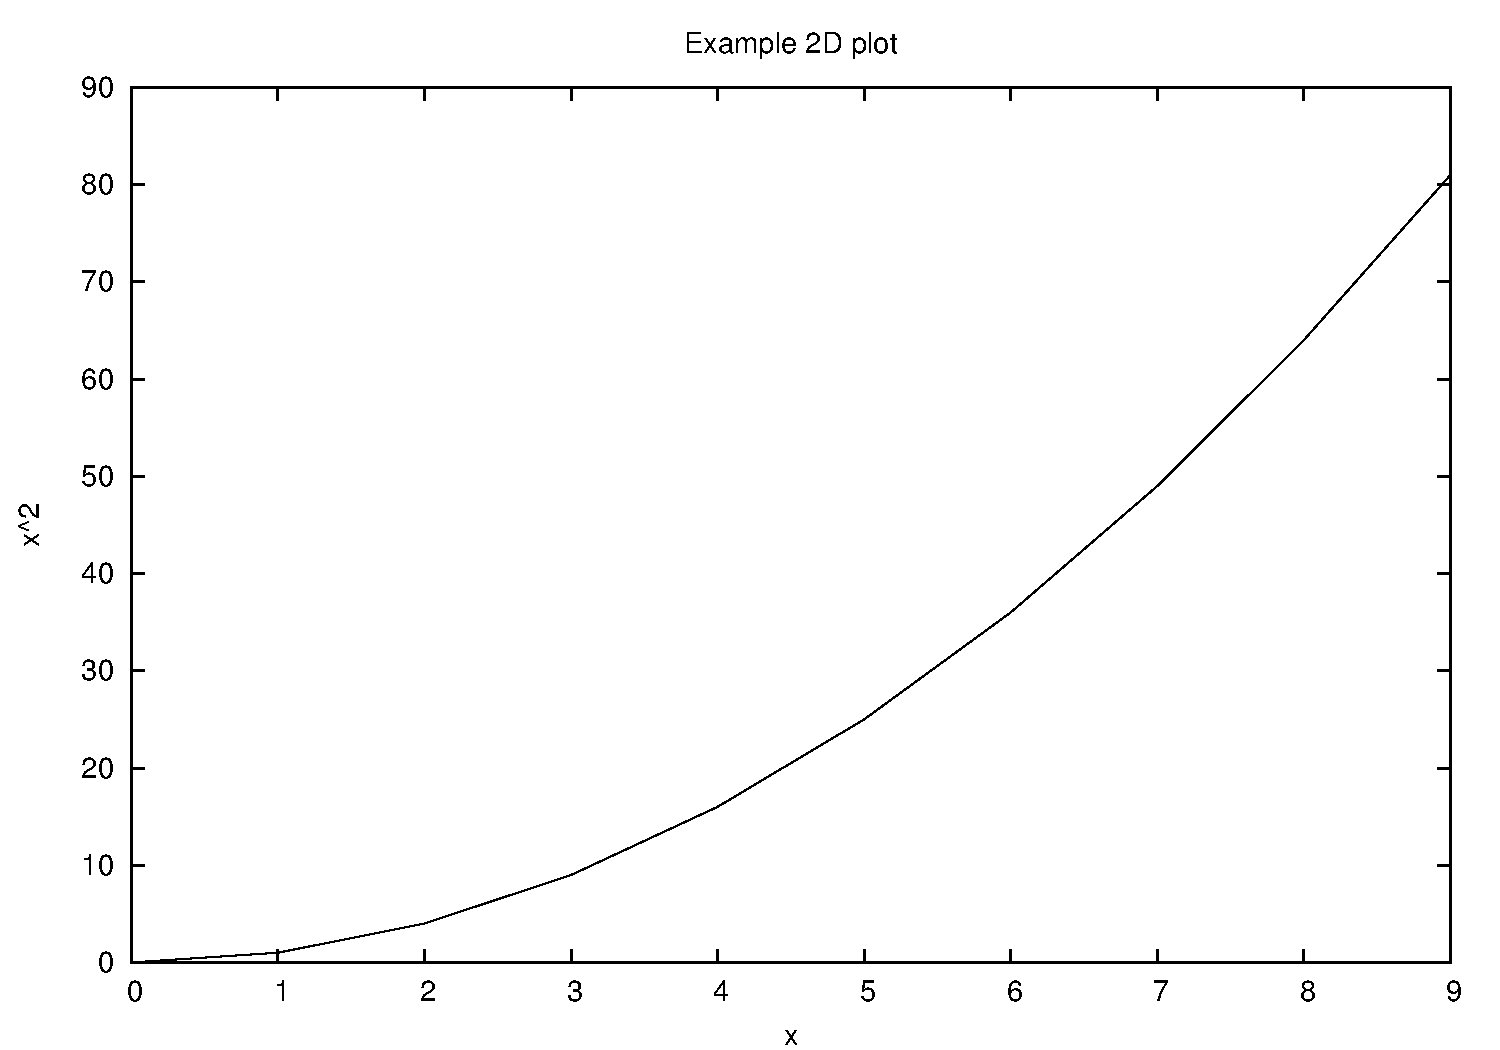
\includegraphics[width=\figwidth]{figures/plotExampleGnuplot}%
}
\caption{Output from gnuplot.}
\end{figure}
\else
\begin{figure}
\centerline{%
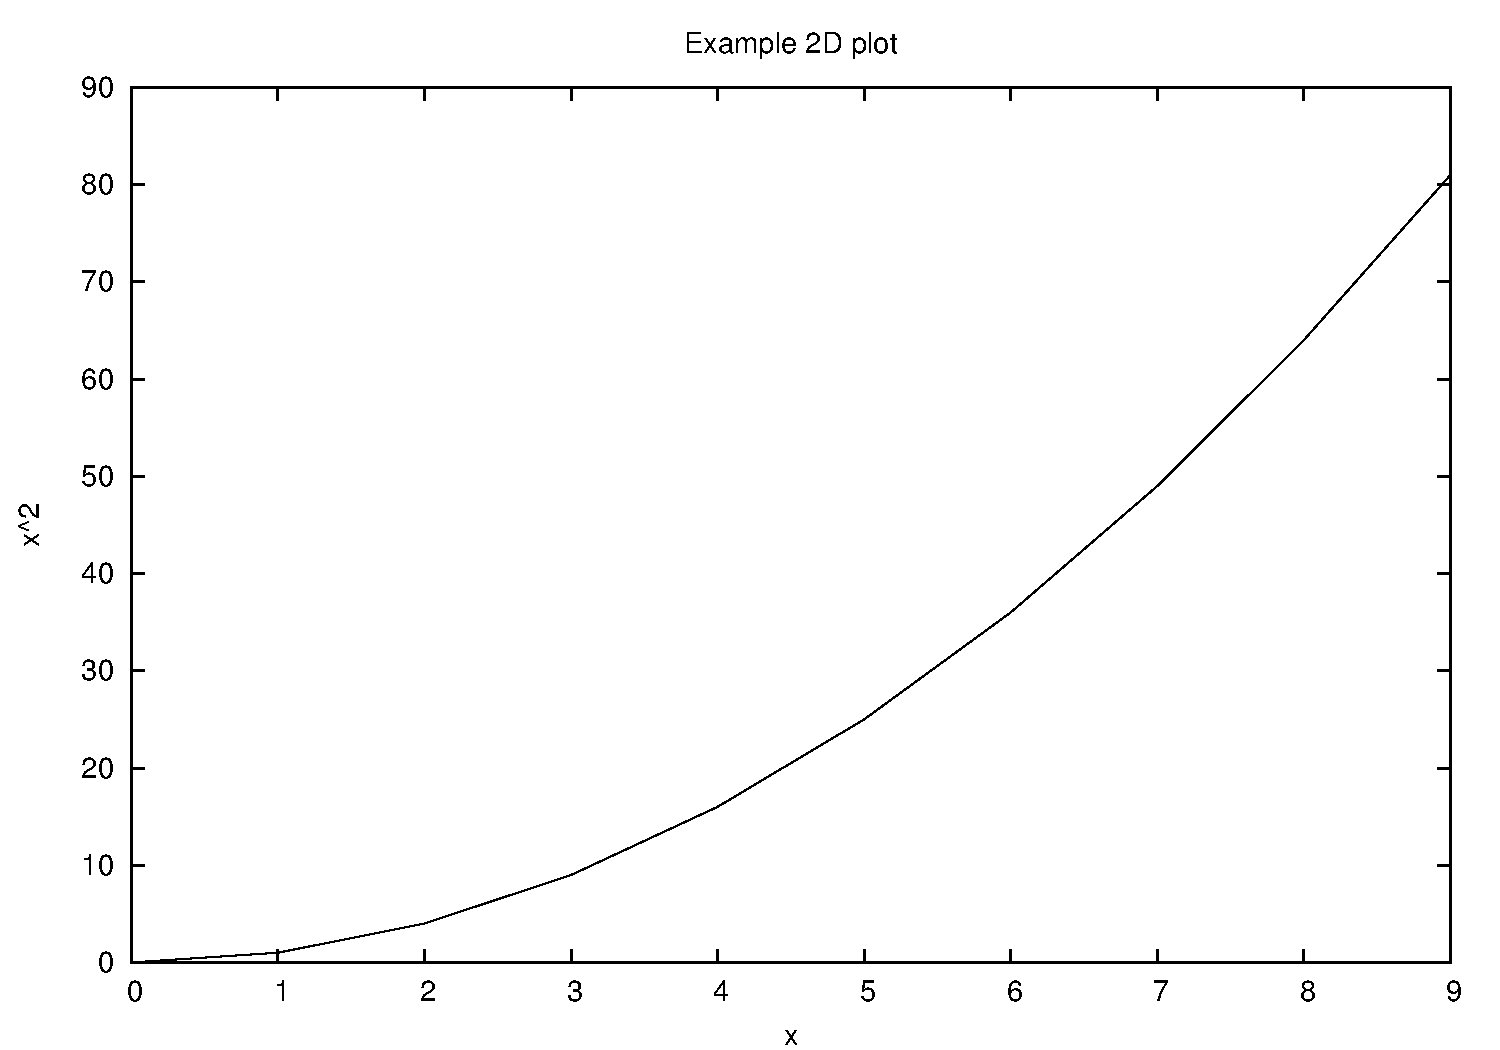
\includegraphics[width=\figwidth,angle=-90]{figures/plotExampleGnuplot}%
}
\caption{Output from gnuplot.}
\end{figure}
\fi

\begin{figure}
\centerline{%
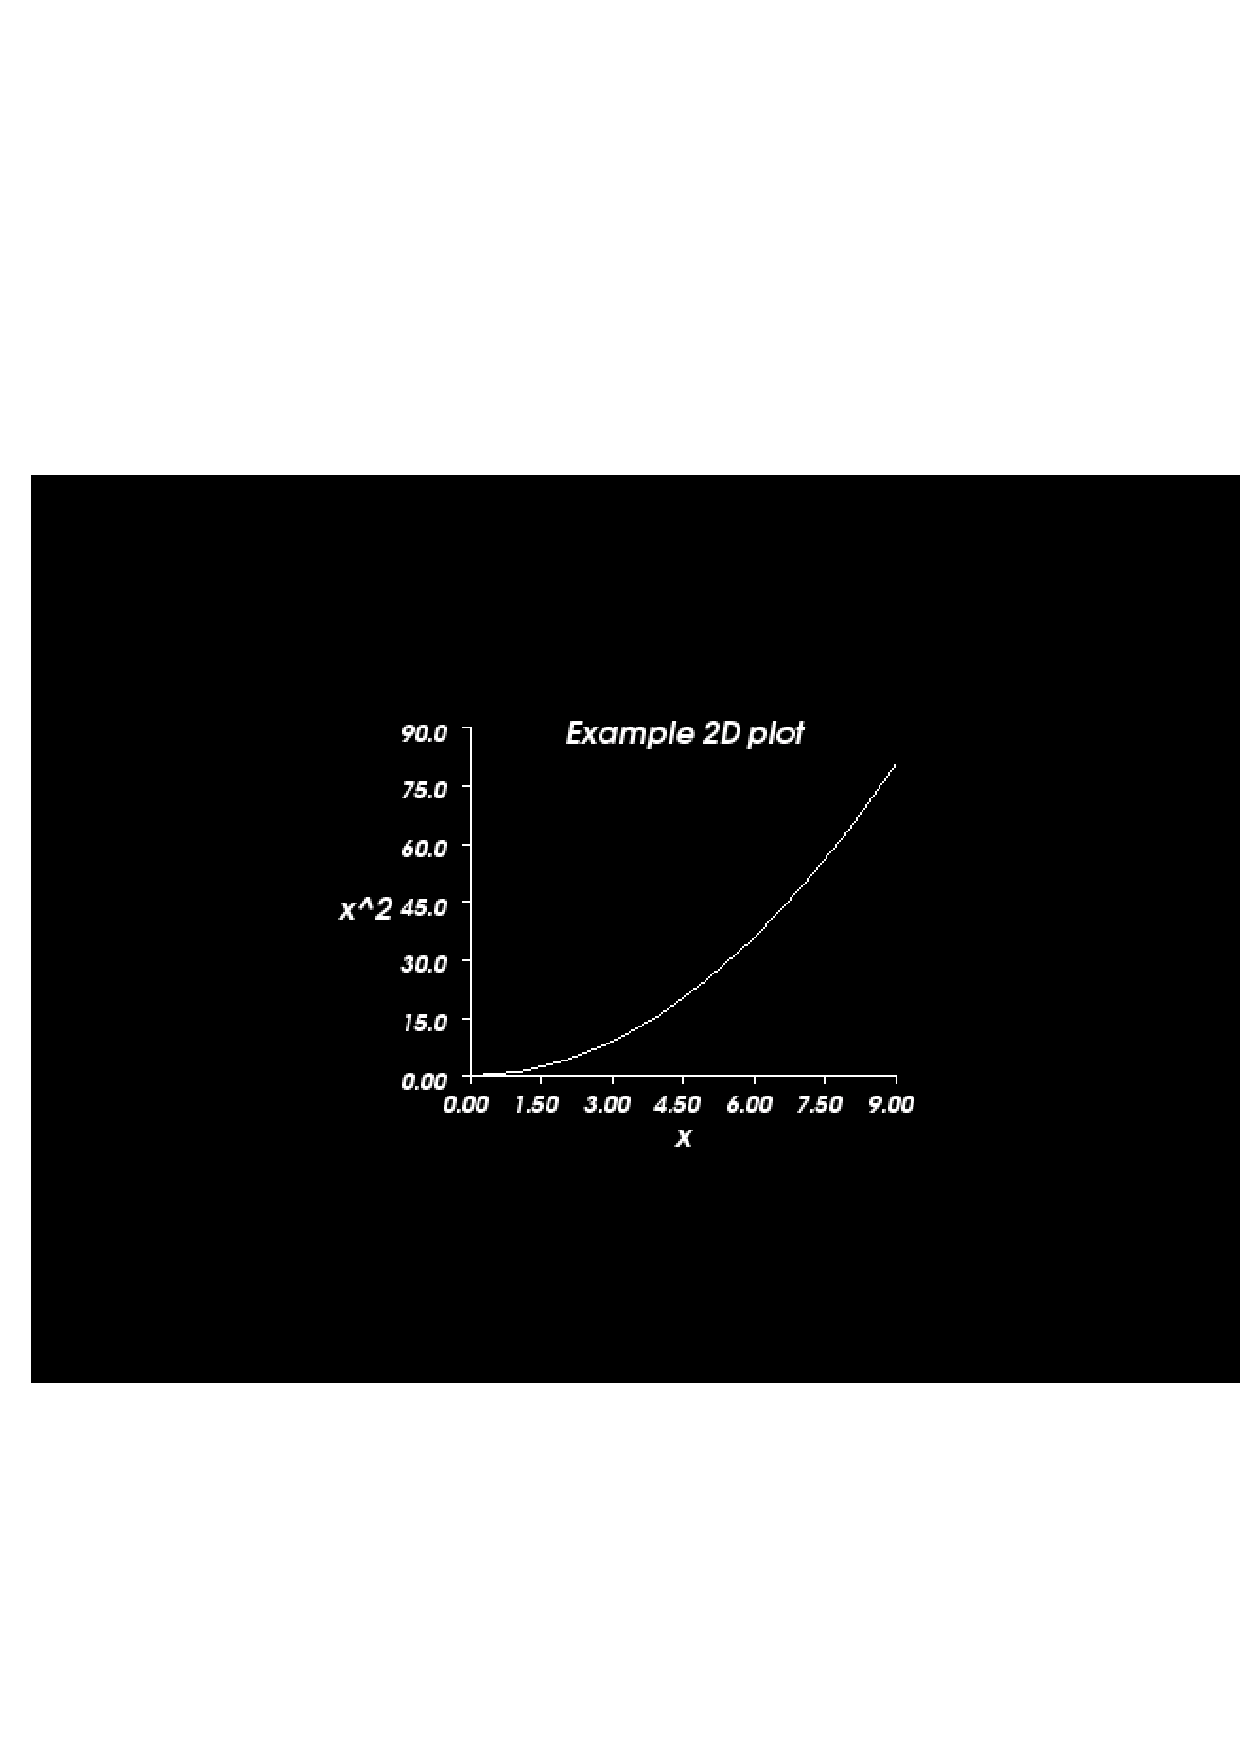
\includegraphics[width=\figwidth]{figures/plotExampleVTK}%
}
\caption{Output from vtk.}
\end{figure}



\part{Reference Manual}
\label{part:languageReference}

% $Id: languageReference.tex,v 1.1 2005/01/12 01:50:54 paultcochrane Exp $

\chapter{Language Reference}
\label{chap:languageRef}



\part{Developer Manual}
\label{part:developerManual}

% $Id: developerManual.tex,v 1.4 2005/02/07 08:09:10 paultcochrane Exp $

\chapter{Developing \pyvisi}
\label{chap:developingPyvisi}

In here should be docs on how people can contribute code, modules, renderers
etc to the pyvisi project.

\chapter{Objects and methods defined at base level}

Developers of \pyvisi renderer modules need to provide the classes, subclasses
and methods described below.  They need to be defined with stub classes or
methods even if that functionality is not supported by the rendering backend.
An error or warning message should be given if the user tries to call these
null methods or classes, however they need to be there for completeness.

The most up to date and complete version of this information is contained on
the \pyvisi web site under the documentation page, and then the API link.

\section{Class structure}

The following figure is the class structure of \pyvisi

\begin{figure}
\centerline{%
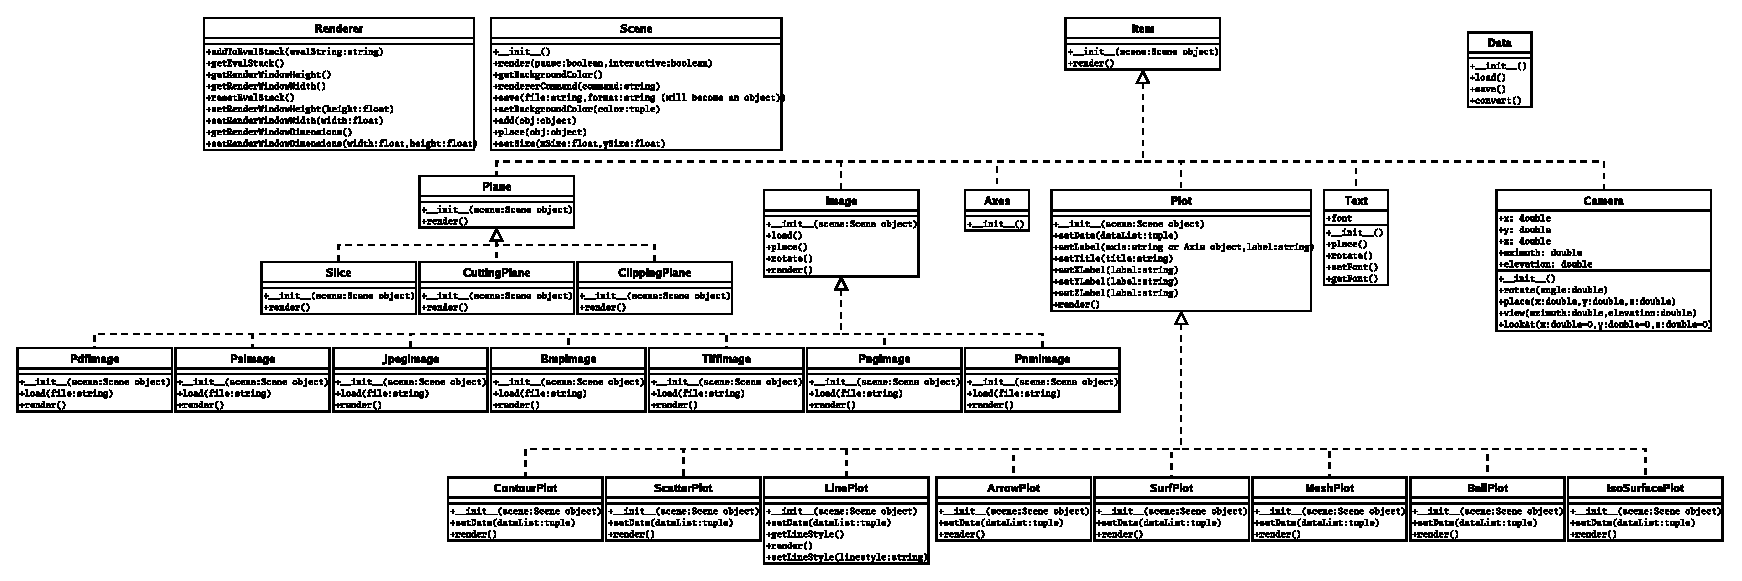
\includegraphics[width=\textheight,angle=90]{figures/pyvisi_class_structure}%
}
\caption{\pyvisi class structure.}
\end{figure}

\section{Fundamental objects}

\subsection{Item}

\subsubsection{render(self)}

Render the object

\subsection{Renderer}

\subsubsection{addToEvalStack(self, evalString)}

Method to add commands to the evaluation stack

\subsubsection{getEvalStack(self)}

Gets the evaluation stack as it currently stands

\subsubsection{getRenderWindowDimensions(self)}

Gets the render window dimensions

\subsubsection{getRenderWindowHeight(self)}

Gets the render window height

\subsubsection{getRenderWindowWidth(self)}

Gets the render window width

\subsubsection{resetEvalStack(self)}

Reset/flush the evaluation stack

\subsubsection{setRenderWindowDimensions(self, width, height)}

Sets the render window dimensions

\subsubsection{setRenderWindowHeight(self, height)}

Sets the render window height

\subsubsection{setRenderWindowWidth(self, width)}

Sets the render window width

\subsection{Scene}

\subsubsection{add(self, obj)}

Add a new item to the scene

\subsubsection{delete(self, obj)}

Delete an item from the scene

\subsubsection{getBackgroundColor(self)}

Gets the current background color setting of the Scene

\subsubsection{getSize(self)}

Gets the current size of the scene

\subsubsection{place(self, obj)}

Place an object within a scene

\subsubsection{render(self, pause, interactive)}

Render (or re-render) the scene

\subsubsection{rendererCommand(self, command)}

Allows the user to run a low-level renderer-specific command directly

\subsubsection{save(self, fname, format)}

Save the scene to a file

\subsubsection{setBackgroundColor(self, *color)}

Sets the background color of the Scene

\subsubsection{setSize(self, xSize, ySize)}

Sets the size of the scene.

\section{Derived objects}

\subsection{Axes}

\subsection{Camera}

\subsection{Image}

\subsubsection{JpegImage}

\subsubsection{PdfImage}

\subsubsection{PngImage}

\subsubsection{PnmImage}

\subsubsection{PsImage}

\subsubsection{TiffImage}

\subsection{Plane}

\subsection{Plot}

\subsubsection{ArrowPlot}

\subsubsection{ContourPlot}

\subsubsection{LinePlot}

\subsection{Text}


%%%%
\chapter{Renderer modules provided by \pyvisi}

\section{vtk}

In the process of being developed.

\section{gnuplot}

In the process of being developed.

\section{povray}

To come.

\section{plplot}

To come.



\part{Appendix}
\label{part:appendix}

\appendix

\chapter{Gnu General Public License}
\label{chap:gpl}

		    GNU GENERAL PUBLIC LICENSE
		       Version 2, June 1991

 Copyright (C) 1989, 1991 Free Software Foundation, Inc.
                       59 Temple Place, Suite 330, Boston, MA  02111-1307  USA
 Everyone is permitted to copy and distribute verbatim copies
 of this license document, but changing it is not allowed.

			    Preamble

  The licenses for most software are designed to take away your
freedom to share and change it.  By contrast, the GNU General Public
License is intended to guarantee your freedom to share and change free
software--to make sure the software is free for all its users.  This
General Public License applies to most of the Free Software
Foundation's software and to any other program whose authors commit to
using it.  (Some other Free Software Foundation software is covered by
the GNU Library General Public License instead.)  You can apply it to
your programs, too.

  When we speak of free software, we are referring to freedom, not
price.  Our General Public Licenses are designed to make sure that you
have the freedom to distribute copies of free software (and charge for
this service if you wish), that you receive source code or can get it
if you want it, that you can change the software or use pieces of it
in new free programs; and that you know you can do these things.

  To protect your rights, we need to make restrictions that forbid
anyone to deny you these rights or to ask you to surrender the rights.
These restrictions translate to certain responsibilities for you if you
distribute copies of the software, or if you modify it.

  For example, if you distribute copies of such a program, whether
gratis or for a fee, you must give the recipients all the rights that
you have.  You must make sure that they, too, receive or can get the
source code.  And you must show them these terms so they know their
rights.

  We protect your rights with two steps: (1) copyright the software, and
(2) offer you this license which gives you legal permission to copy,
distribute and/or modify the software.

  Also, for each author's protection and ours, we want to make certain
that everyone understands that there is no warranty for this free
software.  If the software is modified by someone else and passed on, we
want its recipients to know that what they have is not the original, so
that any problems introduced by others will not reflect on the original
authors' reputations.

  Finally, any free program is threatened constantly by software
patents.  We wish to avoid the danger that redistributors of a free
program will individually obtain patent licenses, in effect making the
program proprietary.  To prevent this, we have made it clear that any
patent must be licensed for everyone's free use or not licensed at all.

  The precise terms and conditions for copying, distribution and
modification follow.

		    GNU GENERAL PUBLIC LICENSE
   TERMS AND CONDITIONS FOR COPYING, DISTRIBUTION AND MODIFICATION

  0. This License applies to any program or other work which contains
a notice placed by the copyright holder saying it may be distributed
under the terms of this General Public License.  The "Program", below,
refers to any such program or work, and a "work based on the Program"
means either the Program or any derivative work under copyright law:
that is to say, a work containing the Program or a portion of it,
either verbatim or with modifications and/or translated into another
language.  (Hereinafter, translation is included without limitation in
the term "modification".)  Each licensee is addressed as "you".

Activities other than copying, distribution and modification are not
covered by this License; they are outside its scope.  The act of
running the Program is not restricted, and the output from the Program
is covered only if its contents constitute a work based on the
Program (independent of having been made by running the Program).
Whether that is true depends on what the Program does.

  1. You may copy and distribute verbatim copies of the Program's
source code as you receive it, in any medium, provided that you
conspicuously and appropriately publish on each copy an appropriate
copyright notice and disclaimer of warranty; keep intact all the
notices that refer to this License and to the absence of any warranty;
and give any other recipients of the Program a copy of this License
along with the Program.

You may charge a fee for the physical act of transferring a copy, and
you may at your option offer warranty protection in exchange for a fee.

  2. You may modify your copy or copies of the Program or any portion
of it, thus forming a work based on the Program, and copy and
distribute such modifications or work under the terms of Section 1
above, provided that you also meet all of these conditions:

    a) You must cause the modified files to carry prominent notices
    stating that you changed the files and the date of any change.

    b) You must cause any work that you distribute or publish, that in
    whole or in part contains or is derived from the Program or any
    part thereof, to be licensed as a whole at no charge to all third
    parties under the terms of this License.

    c) If the modified program normally reads commands interactively
    when run, you must cause it, when started running for such
    interactive use in the most ordinary way, to print or display an
    announcement including an appropriate copyright notice and a
    notice that there is no warranty (or else, saying that you provide
    a warranty) and that users may redistribute the program under
    these conditions, and telling the user how to view a copy of this
    License.  (Exception: if the Program itself is interactive but
    does not normally print such an announcement, your work based on
    the Program is not required to print an announcement.)

These requirements apply to the modified work as a whole.  If
identifiable sections of that work are not derived from the Program,
and can be reasonably considered independent and separate works in
themselves, then this License, and its terms, do not apply to those
sections when you distribute them as separate works.  But when you
distribute the same sections as part of a whole which is a work based
on the Program, the distribution of the whole must be on the terms of
this License, whose permissions for other licensees extend to the
entire whole, and thus to each and every part regardless of who wrote it.

Thus, it is not the intent of this section to claim rights or contest
your rights to work written entirely by you; rather, the intent is to
exercise the right to control the distribution of derivative or
collective works based on the Program.

In addition, mere aggregation of another work not based on the Program
with the Program (or with a work based on the Program) on a volume of
a storage or distribution medium does not bring the other work under
the scope of this License.

  3. You may copy and distribute the Program (or a work based on it,
under Section 2) in object code or executable form under the terms of
Sections 1 and 2 above provided that you also do one of the following:

    a) Accompany it with the complete corresponding machine-readable
    source code, which must be distributed under the terms of Sections
    1 and 2 above on a medium customarily used for software interchange; or,

    b) Accompany it with a written offer, valid for at least three
    years, to give any third party, for a charge no more than your
    cost of physically performing source distribution, a complete
    machine-readable copy of the corresponding source code, to be
    distributed under the terms of Sections 1 and 2 above on a medium
    customarily used for software interchange; or,

    c) Accompany it with the information you received as to the offer
    to distribute corresponding source code.  (This alternative is
    allowed only for noncommercial distribution and only if you
    received the program in object code or executable form with such
    an offer, in accord with Subsection b above.)

The source code for a work means the preferred form of the work for
making modifications to it.  For an executable work, complete source
code means all the source code for all modules it contains, plus any
associated interface definition files, plus the scripts used to
control compilation and installation of the executable.  However, as a
special exception, the source code distributed need not include
anything that is normally distributed (in either source or binary
form) with the major components (compiler, kernel, and so on) of the
operating system on which the executable runs, unless that component
itself accompanies the executable.

If distribution of executable or object code is made by offering
access to copy from a designated place, then offering equivalent
access to copy the source code from the same place counts as
distribution of the source code, even though third parties are not
compelled to copy the source along with the object code.

  4. You may not copy, modify, sublicense, or distribute the Program
except as expressly provided under this License.  Any attempt
otherwise to copy, modify, sublicense or distribute the Program is
void, and will automatically terminate your rights under this License.
However, parties who have received copies, or rights, from you under
this License will not have their licenses terminated so long as such
parties remain in full compliance.

  5. You are not required to accept this License, since you have not
signed it.  However, nothing else grants you permission to modify or
distribute the Program or its derivative works.  These actions are
prohibited by law if you do not accept this License.  Therefore, by
modifying or distributing the Program (or any work based on the
Program), you indicate your acceptance of this License to do so, and
all its terms and conditions for copying, distributing or modifying
the Program or works based on it.

  6. Each time you redistribute the Program (or any work based on the
Program), the recipient automatically receives a license from the
original licensor to copy, distribute or modify the Program subject to
these terms and conditions.  You may not impose any further
restrictions on the recipients' exercise of the rights granted herein.
You are not responsible for enforcing compliance by third parties to
this License.

  7. If, as a consequence of a court judgment or allegation of patent
infringement or for any other reason (not limited to patent issues),
conditions are imposed on you (whether by court order, agreement or
otherwise) that contradict the conditions of this License, they do not
excuse you from the conditions of this License.  If you cannot
distribute so as to satisfy simultaneously your obligations under this
License and any other pertinent obligations, then as a consequence you
may not distribute the Program at all.  For example, if a patent
license would not permit royalty-free redistribution of the Program by
all those who receive copies directly or indirectly through you, then
the only way you could satisfy both it and this License would be to
refrain entirely from distribution of the Program.

If any portion of this section is held invalid or unenforceable under
any particular circumstance, the balance of the section is intended to
apply and the section as a whole is intended to apply in other
circumstances.

It is not the purpose of this section to induce you to infringe any
patents or other property right claims or to contest validity of any
such claims; this section has the sole purpose of protecting the
integrity of the free software distribution system, which is
implemented by public license practices.  Many people have made
generous contributions to the wide range of software distributed
through that system in reliance on consistent application of that
system; it is up to the author/donor to decide if he or she is willing
to distribute software through any other system and a licensee cannot
impose that choice.

This section is intended to make thoroughly clear what is believed to
be a consequence of the rest of this License.

  8. If the distribution and/or use of the Program is restricted in
certain countries either by patents or by copyrighted interfaces, the
original copyright holder who places the Program under this License
may add an explicit geographical distribution limitation excluding
those countries, so that distribution is permitted only in or among
countries not thus excluded.  In such case, this License incorporates
the limitation as if written in the body of this License.

  9. The Free Software Foundation may publish revised and/or new versions
of the General Public License from time to time.  Such new versions will
be similar in spirit to the present version, but may differ in detail to
address new problems or concerns.

Each version is given a distinguishing version number.  If the Program
specifies a version number of this License which applies to it and "any
later version", you have the option of following the terms and conditions
either of that version or of any later version published by the Free
Software Foundation.  If the Program does not specify a version number of
this License, you may choose any version ever published by the Free Software
Foundation.

  10. If you wish to incorporate parts of the Program into other free
programs whose distribution conditions are different, write to the author
to ask for permission.  For software which is copyrighted by the Free
Software Foundation, write to the Free Software Foundation; we sometimes
make exceptions for this.  Our decision will be guided by the two goals
of preserving the free status of all derivatives of our free software and
of promoting the sharing and reuse of software generally.

			    NO WARRANTY

  11. BECAUSE THE PROGRAM IS LICENSED FREE OF CHARGE, THERE IS NO WARRANTY
FOR THE PROGRAM, TO THE EXTENT PERMITTED BY APPLICABLE LAW.  EXCEPT WHEN
OTHERWISE STATED IN WRITING THE COPYRIGHT HOLDERS AND/OR OTHER PARTIES
PROVIDE THE PROGRAM "AS IS" WITHOUT WARRANTY OF ANY KIND, EITHER EXPRESSED
OR IMPLIED, INCLUDING, BUT NOT LIMITED TO, THE IMPLIED WARRANTIES OF
MERCHANTABILITY AND FITNESS FOR A PARTICULAR PURPOSE.  THE ENTIRE RISK AS
TO THE QUALITY AND PERFORMANCE OF THE PROGRAM IS WITH YOU.  SHOULD THE
PROGRAM PROVE DEFECTIVE, YOU ASSUME THE COST OF ALL NECESSARY SERVICING,
REPAIR OR CORRECTION.

  12. IN NO EVENT UNLESS REQUIRED BY APPLICABLE LAW OR AGREED TO IN WRITING
WILL ANY COPYRIGHT HOLDER, OR ANY OTHER PARTY WHO MAY MODIFY AND/OR
REDISTRIBUTE THE PROGRAM AS PERMITTED ABOVE, BE LIABLE TO YOU FOR DAMAGES,
INCLUDING ANY GENERAL, SPECIAL, INCIDENTAL OR CONSEQUENTIAL DAMAGES ARISING
OUT OF THE USE OR INABILITY TO USE THE PROGRAM (INCLUDING BUT NOT LIMITED
TO LOSS OF DATA OR DATA BEING RENDERED INACCURATE OR LOSSES SUSTAINED BY
YOU OR THIRD PARTIES OR A FAILURE OF THE PROGRAM TO OPERATE WITH ANY OTHER
PROGRAMS), EVEN IF SUCH HOLDER OR OTHER PARTY HAS BEEN ADVISED OF THE
POSSIBILITY OF SUCH DAMAGES.

		     END OF TERMS AND CONDITIONS


\part{Bibliography and Index}
\backmatter

\bibliography{pyvisi_doc}
%\printindex

\end{document}

